\documentclass[UTF8,openany]{ctexbook}

% 论文版面要求:
% 统一按 word 格式A4纸(页面设置按word默认值)编排、打印、制作。
% 正文内容字体为宋体;字号为小4号;字符间距为标准;行距为25磅(约0.88175cm)。

%%%%% ===== 页面设置
\usepackage[a4paper,top=2.54cm,bottom=2.54cm,left=3.17cm,right=3.17cm,%
            ]{geometry}
\usepackage{tcolorbox}
\usepackage{colortbl}
\usepackage{dirtree}
\usepackage{longtable}
\usepackage{booktabs}
\usepackage{subfigure}
            
\setlength{\parindent}{2em}
%默认的弹性间距会导致文中某些排版flush的时候,出现大量空白。
\setlength{\parskip}{0.5em} %指定固定段后间距,默认为弹性间距。
\setlength{\intextsep}{10pt} %固定浮浮动体前后间距。
\usepackage{enumitem}
\usepackage{ulem}

%%%%% =====章节 标题 设置
\ctexset{%
  contentsname={\vspace{-3.5em}\centerline{\zihao{-3}\heiti 目\quad 录}\vspace{-0.7em}},
  listfigurename={\vspace{-3.5em}\centerline{\zihao{-3}\heiti 插\ 图\ 目\ 录}\vspace{-0.5em}},
  listtablename={\vspace{-3.5em}\centerline{\zihao{-3}\heiti 表\ 格\ 目\ 录}\vspace{-0.5em}},
  bibname={\vspace{-3em}\centerline{\zihao{-3}\heiti 参\ 考\ 文\ 献}\vspace{3em}},
  chapter={name={,},
  number=\arabic{chapter}, %指定章序号为一二三。。。。
  nameformat={\zihao{-2}\bfseries},
  titleformat={\zihao{-2}\bfseries},
  format=\raggedright,
  beforeskip={10pt},
  afterskip={10pt},
  pagestyle={fancy}
  },
section={format=\raggedright,
  nameformat={\zihao{4}\bfseries},
  titleformat={\zihao{4}\bfseries},
%           afterskip={1ex plus 0.2ex}
  beforeskip={1ex},% 固定段前段后间距,
  afterskip={1ex}
  },
subsection={format=\raggedright,
  nameformat={\zihao{-4}\bfseries},
  titleformat={\zihao{-4}\bfseries},
%           afterskip={0.5ex plus 0.1ex}
  beforeskip={0.5ex},
  afterskip={0.5ex}
  }
}
\AddToHook{package/xeCJK/after}{\defaultCJKfontfeatures{}} % 重置字体设置
%%%%% ===== 中英文字体
%\setsansfont{Myriad Pro} % 无衬线字体 sans serif \sffamily
%\setmonofont{Consolas}   % 等宽字体 typewriter \ttfamily
%\newcommand{\Times}{\fontspec{Times New Roman}}
%% 中文字体
%\setCJKmainfont[BoldFont={Microsoft YaHei},ItalicFont={KaiTi}]{NSimSun}
%\setCJKsansfont{Microsoft YaHei}
%\setCJKmonofont{KaiTi}
% \setCJKfamilyfont{STSong}{方正小标宋_GBK}\newcommand{\STSong}{\CJKfamily{STSong}}
\setCJKfamilyfont{songti}{STZhongsong}\newcommand{\STSong}{\CJKfamily{STSong}}

%%%%% ===== 常用宏包
\usepackage{amsmath,amssymb,amsfonts,bm}
\usepackage[amsmath,thref,thmmarks,hyperref]{ntheorem}
\usepackage{graphicx,xcolor,float}
\usepackage{fancyhdr}

\graphicspath{{img/}}


\usepackage{booktabs} % toprule, midrule, bottomrule
\usepackage{varwidth} % 可变宽度的 parbox

%%%%% ===== 参考文献与链接
\usepackage[numbers,sort&compress,sectionbib,super, square]{natbib} %引用上标,禁用连续缩写。
\newcommand{\upcite}[1]{\textsuperscript{\cite{#1}}}


\usepackage[xetex,pagebackref]{hyperref}
\hypersetup{CJKbookmarks=true,colorlinks=true,citecolor=blue,%
            linkcolor=blue,urlcolor=blue,bookmarksnumbered=true,%
	        bookmarksopen=true,breaklinks=true}
	        
	        
	        
\iffalse   % 调试时,可去掉,以用于显示引用位置。
\renewcommand*{\backrefalt}[4]{%
\ifcase #1 No citations.%
\or Cited on page #2.%
\else Cited on pages #2.%
%\else #1 Cited on pages #2.%
\fi
}

\else
\renewcommand*{\backrefalt}[4]{}
\fi

%%%%% ===== 浮动图表的标题
\usepackage[margin=2em,labelsep=space,skip=0.5em,font=normalfont]{caption}
\DeclareCaptionFormat{mycaption}{{\heiti\color{blue} #1}#2{\kaishu #3}}
\captionsetup{format=mycaption,tablewithin=chapter,figurewithin=chapter}%,belowskip=-10pt
%\setlength{\belowcaptionskip}{-10pt}

%%%%%% ===== 浮动图表的比例默认50%以下,否则无法浮动。
\renewcommand\floatpagefraction{.9} %当浮动体小于页面90%时进行直接放置。
\renewcommand\topfraction{.9}  
\renewcommand\bottomfraction{.9}  
\renewcommand\textfraction{.1}



%%%%% ===== 算法
\usepackage{algorithm,algpseudocode}

%%%%% ===== 其他
\usepackage{ulem}
\def\ULthickness{1pt}




%%%%%===== Code Style代码
\usepackage{listings}
\usepackage{color}

\definecolor{dkgreen}{rgb}{0,0.6,0}
\definecolor{gray}{rgb}{0.5,0.5,0.5}
\definecolor{mauve}{rgb}{0.58,0,0.82}

\usepackage{accsupp}



\newcommand\emptyaccsupp[1]{\BeginAccSupp{ActualText={}}#1\EndAccSupp{}}

\lstset{
    % language = C,
    showstringspaces=false,
    xleftmargin = 3em,xrightmargin = 3em, aboveskip = 1em,
	backgroundcolor = \color{white}, % 背景色
	basicstyle = \small\ttfamily, % 基本样式 + 小号字体
	rulesepcolor= \color{gray}, % 代码块边框颜色
	breaklines = true, % 代码过长则换行
	numbers = left, % 行号在左侧显示
	numberstyle=\emptyaccsupp,
    numbersep = 14pt, 
    keywordstyle=\color{purple}\bfseries, % 关键字颜色
    commentstyle =\color{red!50!green!50!blue!60}, % 注释颜色
    stringstyle = \color{red}, % 字符串颜色
    morekeywords={ASSERT, int64_t, uint32_t},
	% frame = shadowbox, % 用(带影子效果)方框框住代码块
	frame = single, % 用(带影子效果)方框框住代码块
	showspaces = false, % 不显示空格
	columns = fixed, % 字间距固定
  framesep=1em
} 
\lstset{
    sensitive=true,
    moreemph={ASSERT, NULL}, emphstyle=\color{red}\bfseries,
    moreemph=[2]{int64_t, uint32_t, tid_t, uint8_t, int16_t, uint16_t, int32_t, size_t}, emphstyle=[2]\color{purple}\bfseries,
    showspaces = false, % 不显示空格
    }



\newcommand{\mcc}[1]{\multicolumn{1}{c}{\underline{\makebox[10em][c]{#1}}}}
\newcommand{\mce}[1]{\multicolumn{1}{c}{\underline{\makebox[15em][l]{#1}}}}


\pagestyle{fancy}
\fancyhf{}  % 清除以前对页眉页脚的设置

\newcommand{\makeheadrule}{%% 定义页眉与正文间双隔线
    \makebox[0pt][l]{\rule[.7\baselineskip]{\headwidth}{0.3pt}}%0.4
    \rule[0.85\baselineskip]{\headwidth}{1.0pt}\vskip-.8\baselineskip}
\makeatletter
\renewcommand{\headrule}{%
    % {\if@fancyplain\let\headrulewidth\plainheadrulewidth\fi\makeheadrule}}
    {\makeheadrule}}
\makeatother
\renewcommand{\chaptermark}[1]{\markboth{\CTEXthechapter \ #1}{}}
\renewcommand{\sectionmark}[1]{\markright{\thesection \ #1}{}}
%\fancyhead[RO,LE]{{\small\songti\rightmark}}     % 节标题
%\fancyhead[RE]{{\small\songti\leftmark}}      % 章标题
\fancyhead[C]{《智能计算系统》课程期中项目报告}
% \fancyhead[RO,LE]{$\cdot$ {\small\thepage} $\cdot$}
\fancyfoot[C]{{-\thepage-}}
%\fancyfoot[CO,CE]{{\thepage}}

\ctexset{chapter/break={}}

\begin{document}

\begin{titlepage}
    \begin{center}

        {
            \begin{figure}[H]
                \vspace{5cm}
                
\includegraphics[width=14cm]{0.png}
            \end{figure}
            \heiti\zihao{2}《智能计算系统》课程期中项目报告\\
            \vspace{1.8em}
            
        }
        
        \zihao{-3}
        \begin{tabular}{p{0cm}p{0em}@{\extracolsep{0.5ex}}cc}
            ~ & \hfill             &  & \mcc{武泽恺\quad 10225101429}      \\
             & \hfill             &  & \url{https://github.com/Mingle-2012/style-transfer} \\
        \end{tabular}
        \\[8em]
        \zihao{-2}2025年5月
    \end{center}
    \thispagestyle{fancy}
    \fancyfoot[C]{}
\end{titlepage}
\fancyfoot[C]{-\thepage-}

\setcounter{page}{1}
\pagenumbering{roman}

\thispagestyle{fancy}
\newpage

\setcounter{page}{1}
\pagenumbering{arabic}

\begin{center}
    \zihao{-2}\heiti 图像风格迁移任务
\end{center}

\chapter{实验概述}

\section{实验目的}

图像风格迁移根据给定的目标风格图像和目标内容图像求解风格迁移图像,使风格迁移图像在风格上与目标风格图像一致,在内容上与目标内容图像一致。

本实验的目的是通过掌握深度学习的训练方法,实现风格迁移模型的训练。一般的风格迁移任务在进行训练时,首先输入图像到图像转换网络生成风格化图像,再利用特征提取网络计算内容损失和风格损失,然后迭代地更新图像转换网络生成风格化图像,再利用特征提取网络计算内容损失和风格损失,然后迭代地更新图像转换网络的参数以最小化损失。

\section{实验内容}

根据实验教程,运用 Imagenet 数据集训练出一个能实现风格迁移的模型(目标风格图像类型可以自选),并输出该模型的内容损失 $content\_loss$ 或风格重建损失 $style\_loss$,同时给出对图像进行风格迁移的时间 $delta\_time$,根据指标作为评判标准。

\section{实验要求}

\begin{enumerate}
    \item 风格迁移时间不得过长。
    \item 需要提交一份实验报告,不少于 3 页,内容包括:所使用的神经网络模型详情、所使用的模型中的亮点、最终风格迁移过程中的损失值。
\end{enumerate}

\chapter{实验过程}

我们首先在\textsection\ref{sec:dataset}中介绍数据集的准备工作,然后在\textsection\ref{sec:env}中介绍实验环境的配置,接着在\textsection\ref{sec:model}中介绍我们所采用的模型。

\section{数据集准备}
\label{sec:dataset}

风格迁移任务需要准备内容图像数据集和风格图像数据集。根据实验要求,我们采用了 Imagenet~\cite{deng2009imagenet} 作为内容图像数据集,包含了多种类型的图像。然而,由于原始的 Imagenet 数据集十分庞大,本次实验所使用的设备条件可能无法承受高强度的训练,因此我们采用了 Kaggle 上开源的 Imagenet (mini)~\footnote{\url{https://www.kaggle.com/datasets/ifigotin/imagenetmini-1000}} 数据集,即使用从原始的Imagenet数据集中采样的小型数据集来进行训练。对于风格数据集,我们采用了开源的动漫风格数据集 Shinkai~\cite{Liu2024dtgan},该数据集包含了新海诚的电影《君の名は。》中的大量动漫风格图像。具体信息如表~\ref{tab:dataset}所示。

\begin{table}[H]
    \centering
    \caption{数据集信息}
    \label{tab:dataset}
    \begin{tabular}{ccccc}
        \toprule
        数据集名称 & 数据集类型 & 数据集大小 & 图片数量 & 来源 \\ \midrule
        Imagenet~\cite{deng2009imagenet}  & 混合 & 3.48 GB & 34745 & Kaggle   \\
        Shinkai~\cite{Liu2024dtgan}  & 动漫 & 137 MB & 1445 & Github  \\ \bottomrule
    \end{tabular}
\end{table}

\begin{figure}[ht!]
    \centering
    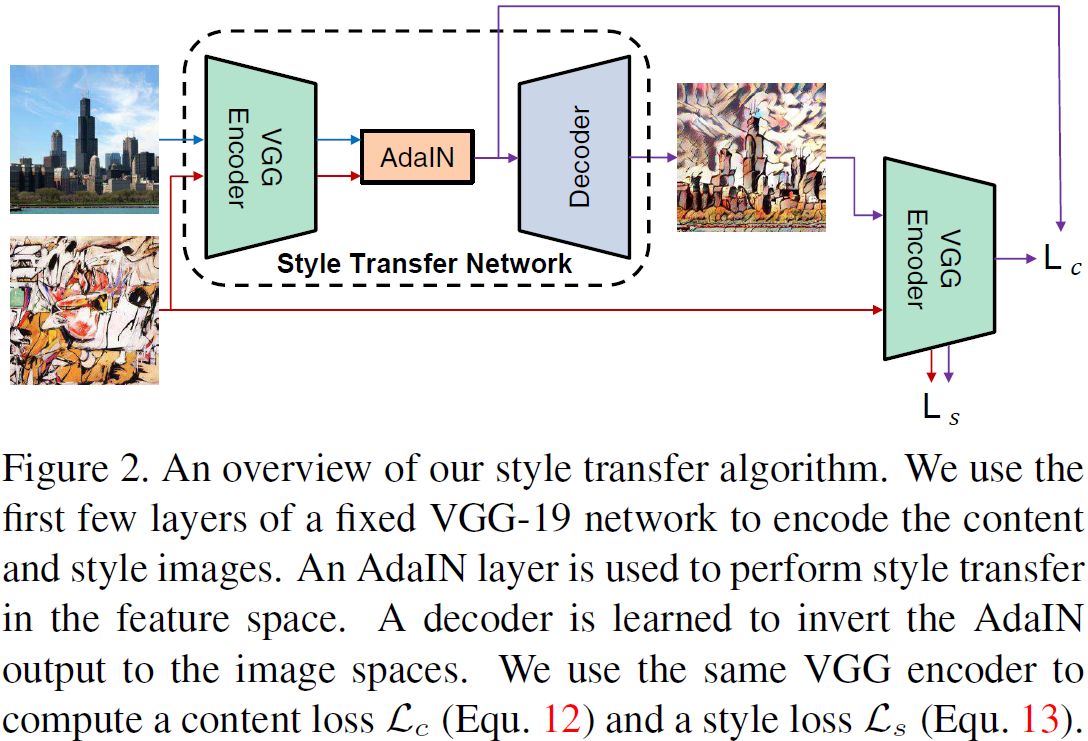
\includegraphics[width=0.8\textwidth]{1.png}
    \caption{模型架构图\cite{huang2017arbitrary}}
    \label{fig:model}
\end{figure}

\section{实验环境}
\label{sec:env}

本实验中,我们使用 PyTorch 框架在具备 GPU 加速的环境下进行风格迁移模型的训练。具体实验环境配置如表~\ref{tab:env}所示。

\begin{table}[H]
    \centering
    \caption{实验环境配置}
    \label{tab:env}
    \begin{tabular}{cc}
        \toprule
        环境配置项 & 配置值 \\ \midrule
        操作系统 & Ubuntu 22.04 LTS \\
        CPU 型号 & Intel(R) Core(TM) i7-12700H CPU @ 2.30GHz \\
        RAM 大小 & 32 GB \\
        Python 版本 & 3.9.21 \\
        PyTorch 版本 & 2.7.0+cu118 \\
        torchvision 版本 & 0.22.0+cu118 \\
        CUDA 版本 & 11.5 \\
        GPU 型号 & NVIDIA GeForce RTX 3070ti, 显存 8GB \\
        NVIDIA 驱动版本 & 561.19 \\ 
        开发环境 & Visual Studio Code \\ 
        主要依赖库 & numpy, tqdm \\ \bottomrule
    \end{tabular}
\end{table}

\section{模型训练}
\label{sec:model}

本实验采用了一种基于自适应实例归一化 (Adaptive Instance Normalization, AdaIN \cite{huang2017arbitrary}) 的深度学习模型进行图像风格迁移,架构为编码器-解码器模型,模型架构图如图~\ref{fig:model}所示。

模型的输入为内容图像和风格图像,经过VGG19编码器提取特征后,使用 AdaIN 进行风格迁移,最后通过解码器生成风格化图像。模型训练流程如图~\ref{fig:model2}所示。

\begin{figure}[ht!]
    \centering
    \hspace*{2.5cm}
    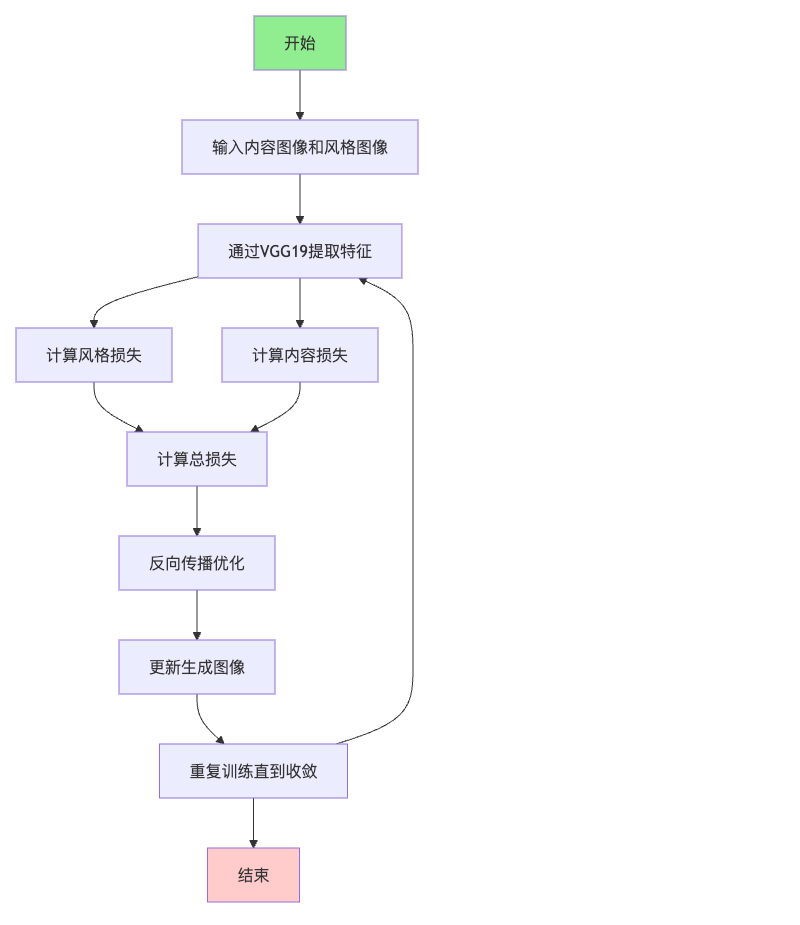
\includegraphics[width=1.0\textwidth]{flow}
    \caption{模型训练流程图}
    \label{fig:model2}
\end{figure}

\subsection{编码器}

编码器部分使用了预训练的VGG19模型,VGG19是经典的卷积神经网络,通常用于图像分类和特征提取。本实验中裁剪了VGG19模型的前21层,仅保留了其中用于提取图像高层语义信息的部分(主要是卷积层)。编码器从内容图像和风格图像中提取特征,即relu1\_1, relu2\_1, relu3\_1, relu4\_1这四个中间层,这些特征用于后续的内容损失和风格损失计算。

\subsection{AdaIN}

核心的风格迁移技术是自适应实例归一化(AdaIN\cite{huang2017arbitrary})。AdaIN通过归一化内容图像的特征,并将其与风格图像的特征进行匹配。论文中所提出的公式如~\ref{eq:adain}所示,内容图像的特征被标准化(减去均值并除以标准差),然后通过风格图像的均值和标准差进行反标准化,从而实现内容图像的结构与风格图像的风格信息的融合。该操作使得生成图像能够在保持内容结构的同时,融合风格图像的色调、纹理等风格特征。

\begin{equation}
    \text{AdaIN}(x, y) = \sigma(y) \left( \frac{x - \mu(x)}{\sigma(x)} \right) + \mu(y)
    \label{eq:adain}
\end{equation}

其中,$x$ 是内容图像的特征,$y$ 是风格图像的特征,$\mu(x)$ 和 $\sigma(x)$ 分别是内容图像特征的均值和标准差,$\mu(y)$ 和 $\sigma(y)$ 分别是风格图像特征的均值和标准差。

\subsection{解码器}

解码器基于逐层恢复的思想,通过反复卷积和上采样操作,逐步增强图像细节。这一部分负责将经过AdaIN处理后的特征恢复为完整的图像,由多个卷积层和上采样层组成,通过逐步还原特征图的空间信息,最终生成与输入图像相同尺寸的输出图像。

\subsection{损失函数}

在本实验中,我们使用了两种损失函数来评估生成图像的质量:内容损失和风格损失。

\begin{itemize}[nosep]
    \item \textbf{内容损失}:通过计算生成图像与内容图像在编码器特征空间中的差异,来保持图像的内容结构。内容损失使用均方误差(MSE)来度量内容图像与生成图像在VGG19最后一层特征的差异。
    \item \textbf{风格损失}:通过计算生成图像和风格图像在多个中间层(relu1\_1, relu2\_1,relu3\_1, relu4\_1)上的特征的均值和标准差的差异,来保持风格图像的纹理和色调。风格损失也是通过MSE计算的。
\end{itemize}

最终的优化目标是最小化内容损失和风格损失的加权和,如公式~\ref{eq:loss}所示:

\begin{equation}
    \mathcal{L} = \mathcal{L}_c + \lambda \mathcal{L}_s
    \label{eq:loss}
\end{equation}

其中,$\mathcal{L}_c$ 是内容损失,$\mathcal{L}_s$ 是风格损失,$\lambda$ 是风格损失的权重系数。

在训练过程中,我们使用Adam优化器来更新模型参数,学习率设置为0.00005。训练过程中,我们每隔一定的迭代次数保存一次模型,并记录当前的内容损失和风格损失。

\subsection{模型亮点}

本实验所采用的模型亮点有以下几点:

\begin{itemize}[nosep]
    \item \textbf{通过统计匹配实现风格迁移:} AdaIN的核心机制是将内容图像的特征图与风格图像的统计量(均值和方差)对齐,从而实现风格迁移。通过这种方式,模型能够在保持内容图像结构的同时,灵活地应用不同风格图像的风格特征。
    \item \textbf{任意风格迁移:} 相比早期方法\cite{gatys2016image},每个风格训练一个模型,AdaIN支持任意风格图在一次前向传播中迁移到内容图像。
    \item \textbf{架构简单高效:} AdaIN 风格迁移模型的架构相对简单,主要由编码器、AdaIN层和解码器组成,这样的架构训练简单,推理速度快于早期方法\cite{gatys2016image}。
\end{itemize}

\begin{figure}[h!]
    \centering
    \subfigure[$\lambda = \frac{1}{3}$]{
        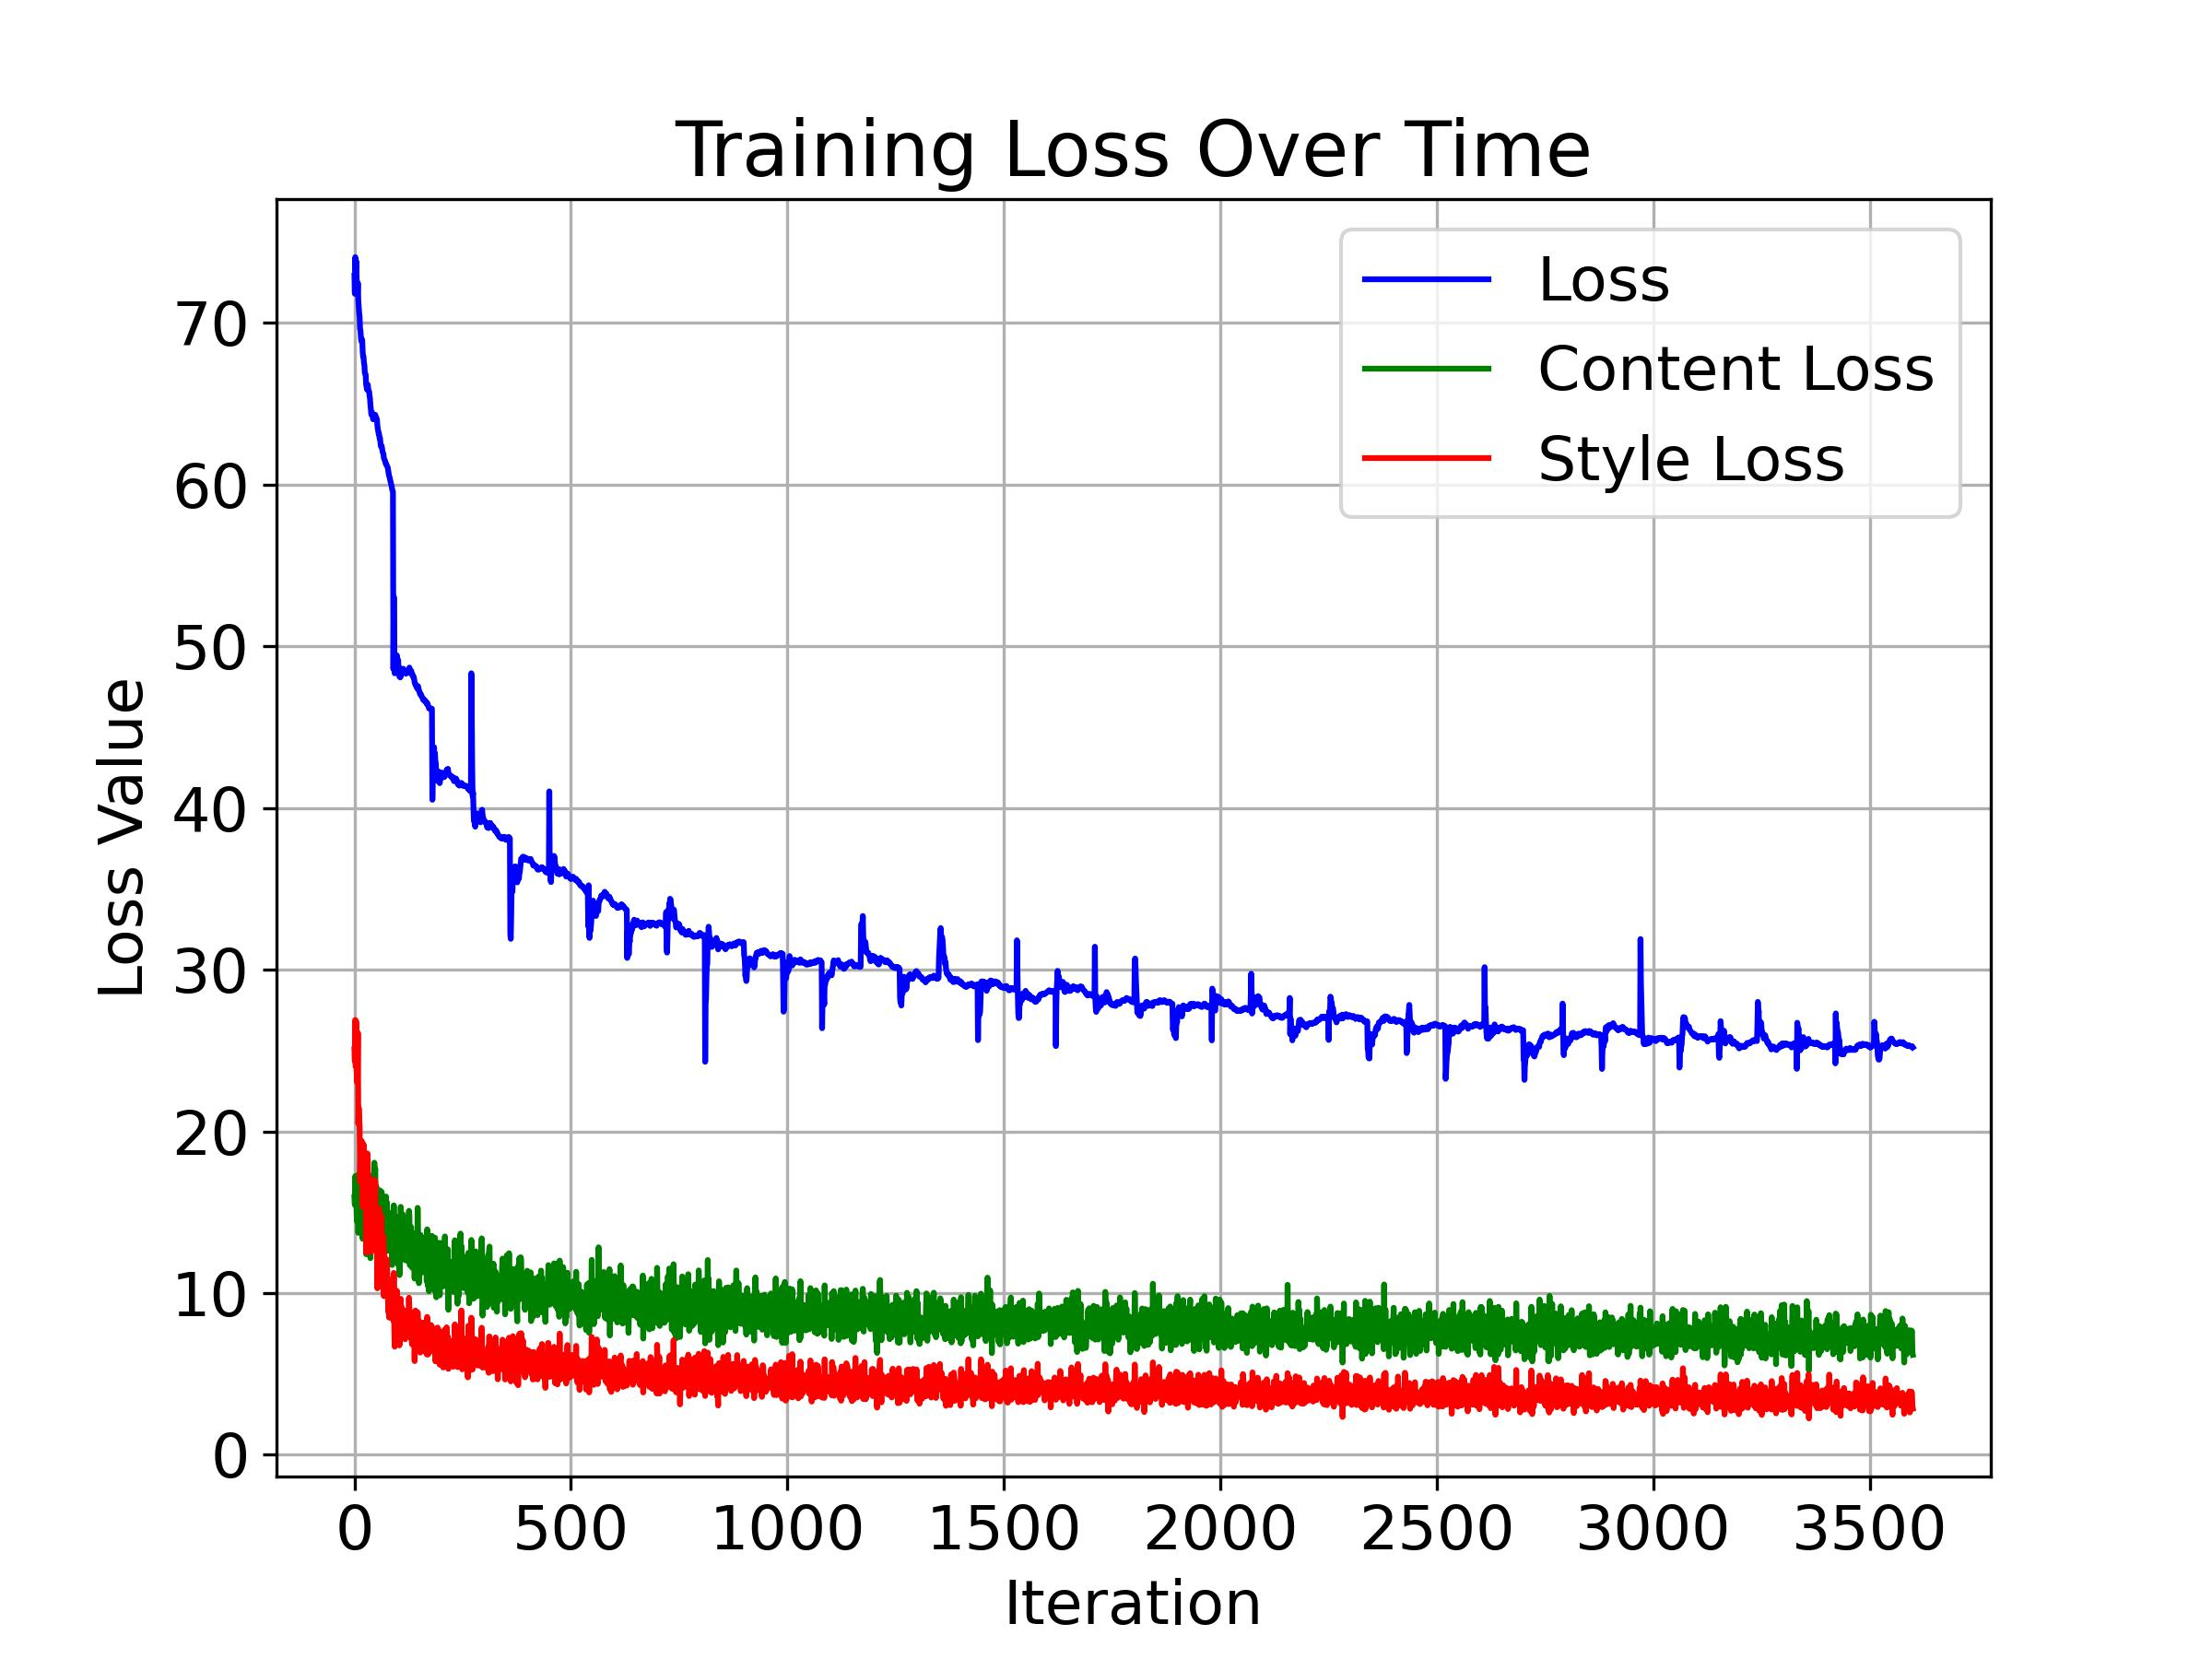
\includegraphics[width=0.47\textwidth]{content3.jpg}
    }
    \subfigure[$\lambda = 1$]{
        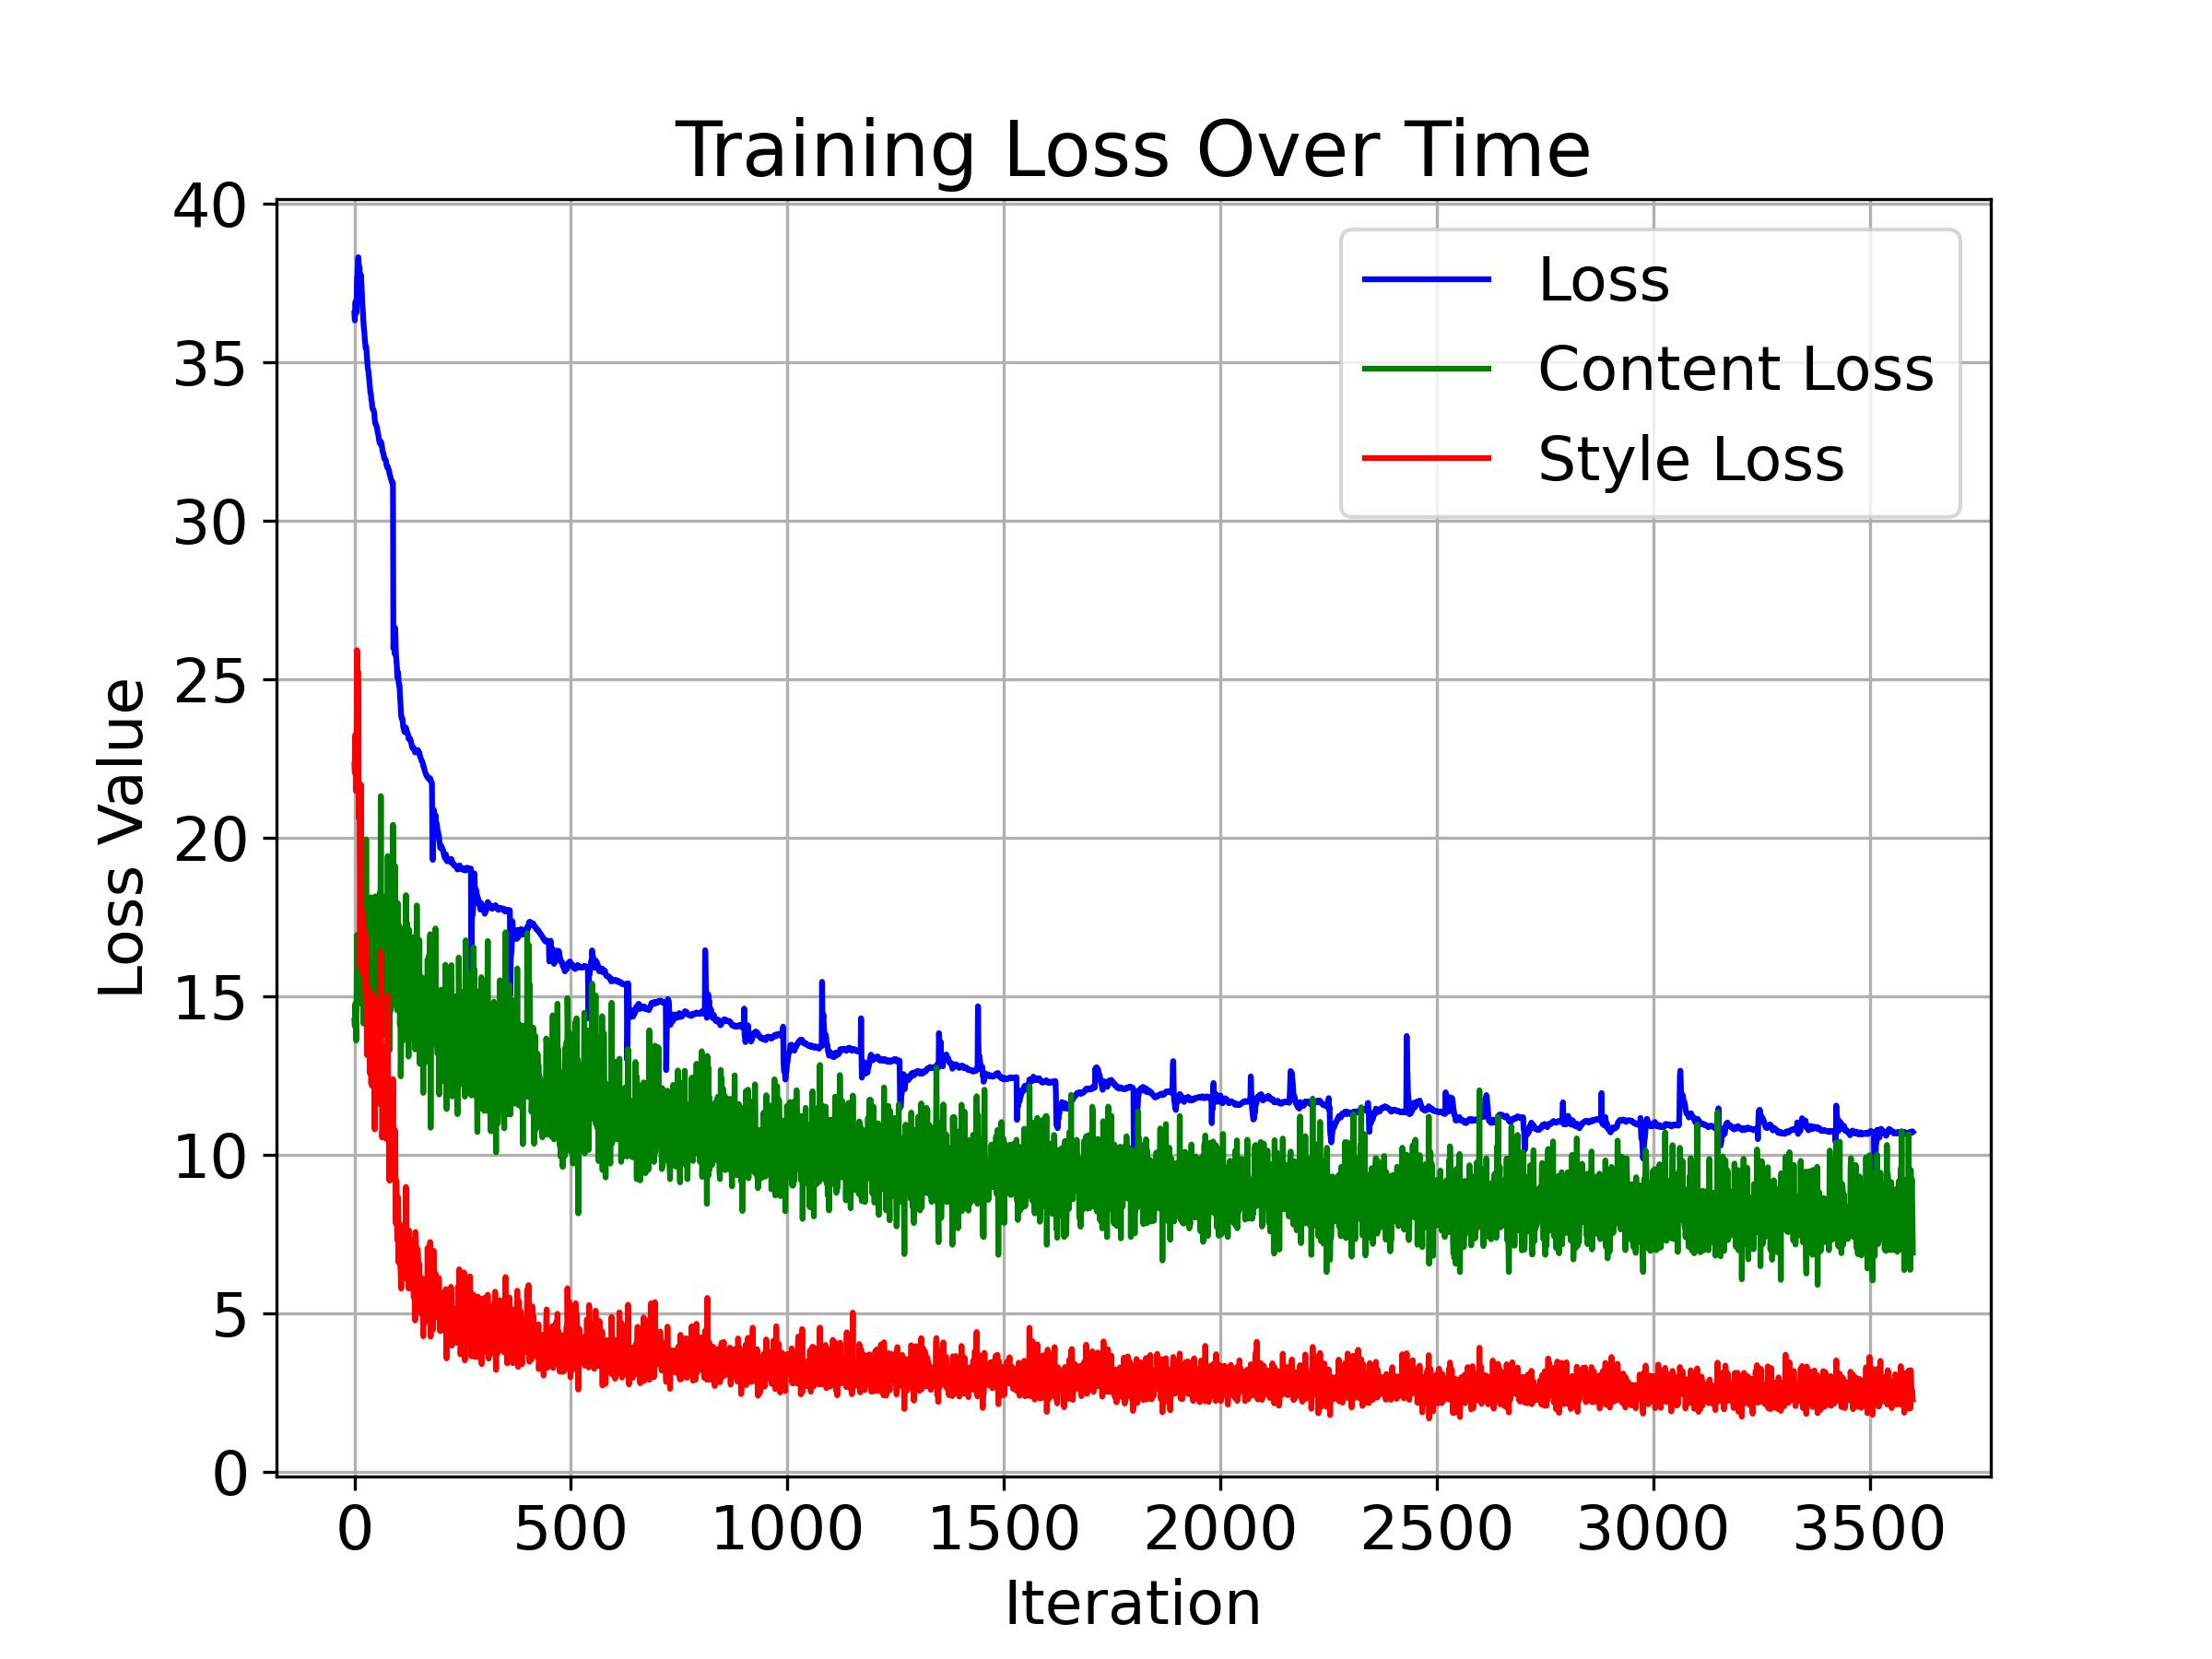
\includegraphics[width=0.47\textwidth]{style1.jpg}
    }
    \subfigure[$\lambda = 3$]{
        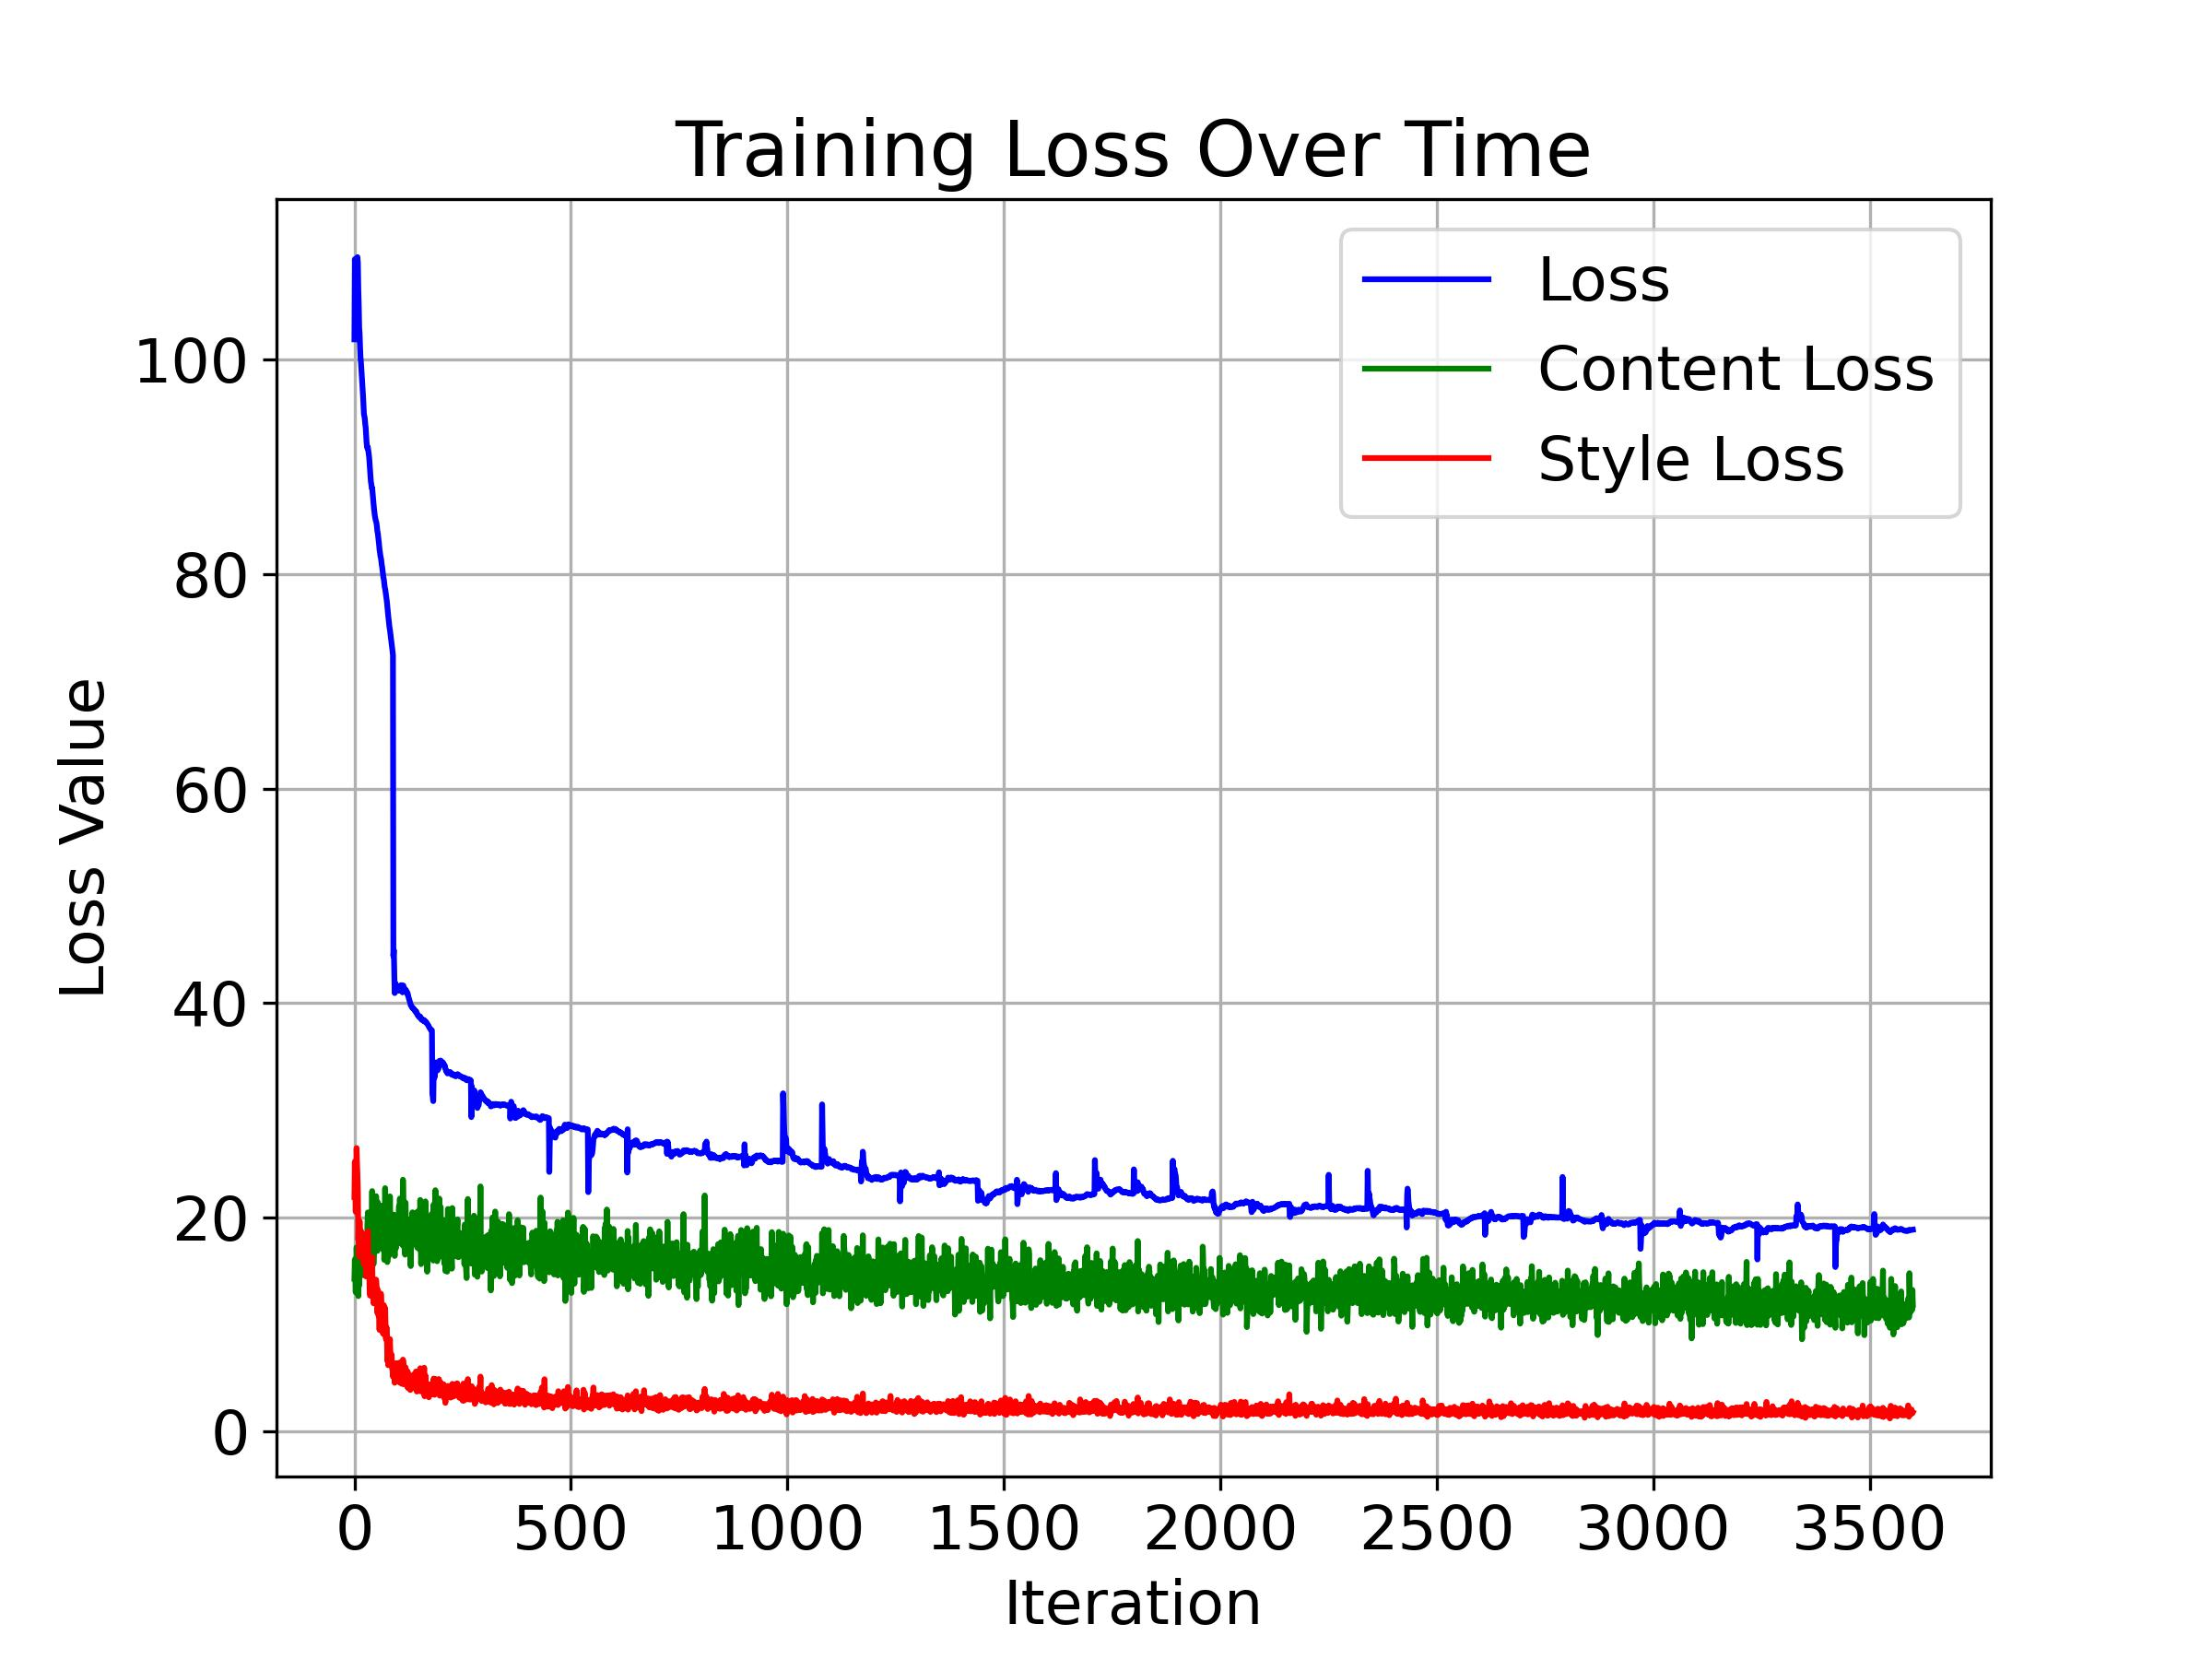
\includegraphics[width=0.47\textwidth]{style3.jpg}
    }
    \subfigure[$\lambda = 10$]{
        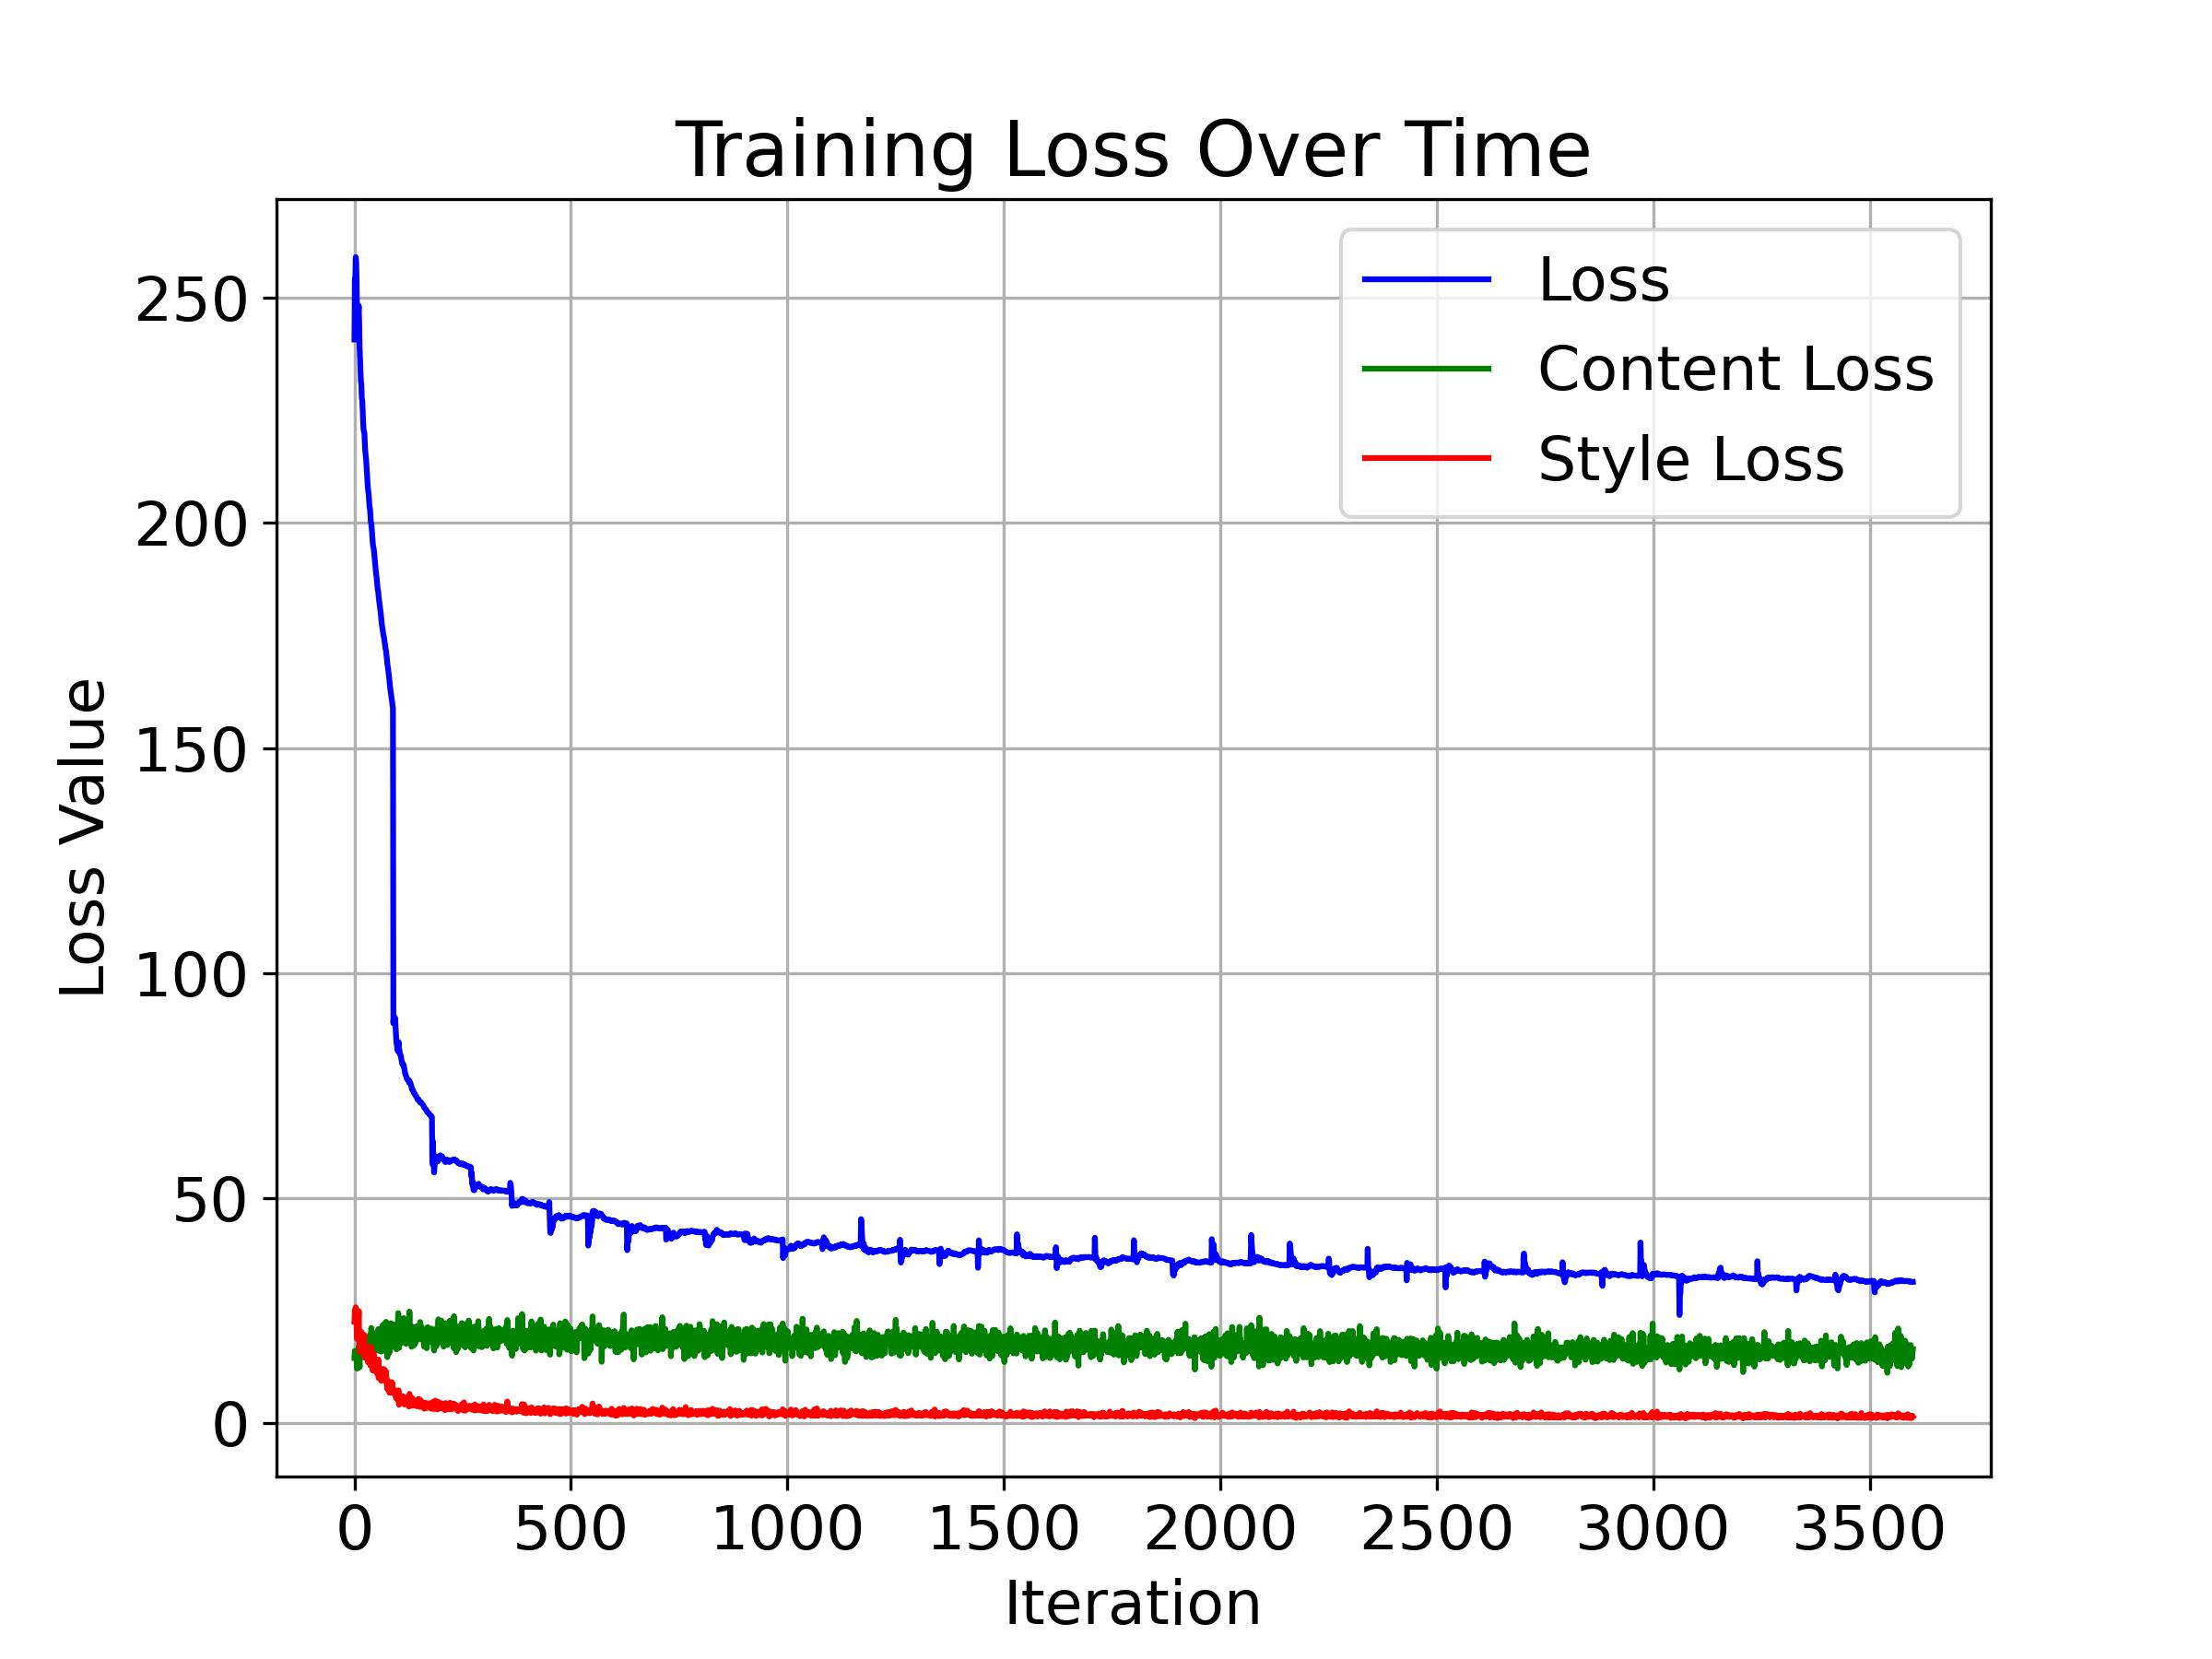
\includegraphics[width=0.47\textwidth]{style10.jpg}
    }
    \caption{不同 $\lambda$ 值下的总损失曲线$\mathcal{L}_\lambda$}
    \label{fig:loss}
\end{figure}

\begin{table}[h!]
    \centering
    \caption{不同 $\lambda$ 下的训练时间(秒)}
    \begin{tabular}{ccccc}
        \toprule
        $\lambda$ & $\frac{1}{3}$ & 1 & 3 & 10 \\
        \midrule
        训练时间$t$ & 2321.24 & 2129.29  & 2556.45 & 2619.18 \\
        最终损失值 & 25.1919 & 10.7254 & 18.8458 & 31.4229 \\
        \bottomrule
    \end{tabular}
    \label{tab:lambda_time_transposed}
\end{table}

\chapter{实验结果}

\section{代码实现}

本实验的代码仓库已开源在Github上,地址为\url{https://github.com/Mingle-2012/style-transfer}。其中,模型代码位于\texttt{model.py}文件中,训练代码位于\texttt{train.py}文件中,风格迁移代码位于\texttt{stylize.py}文件中,\texttt{readme}文件也提供了使用说明便于复现。

\begin{figure}[h!]
    \centering
    \subfigure[风格图像1]{
        
\includegraphics[width=0.32\textwidth]{styles1.png}
    }
    \subfigure[风格图像2]{
        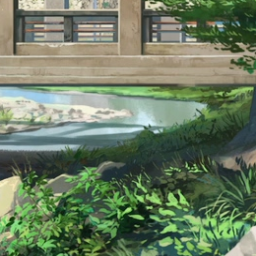
\includegraphics[width=0.32\textwidth]{styles2.png}
    }
    \caption{两个来自动漫风格数据集的风格图像}
    \label{fig:styles}
\end{figure}

\begin{figure}[h!]
    \centering
    \subfigure[原内容图像]{
        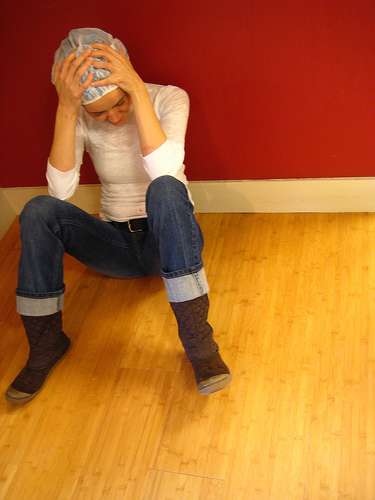
\includegraphics[width=0.17\textwidth]{content1.jpg}
    }
    \subfigure[$\lambda = \frac{1}{3}$]{
        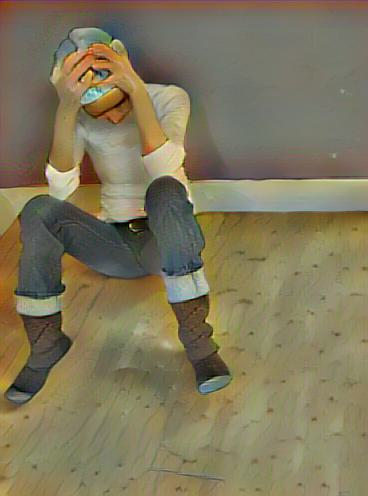
\includegraphics[width=0.17\textwidth]{content1_style1_content3.jpg}
    }
    \subfigure[$\lambda = 1$]{
        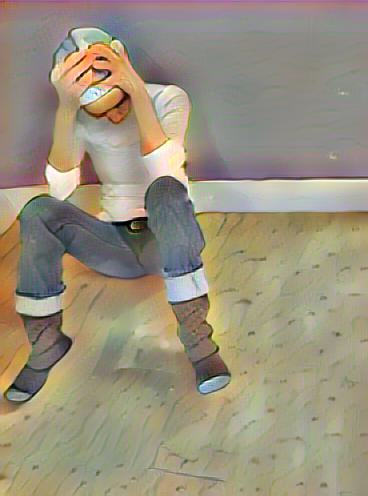
\includegraphics[width=0.17\textwidth]{content1_style1_style1.jpg}
    }
    \subfigure[$\lambda = 3$]{
        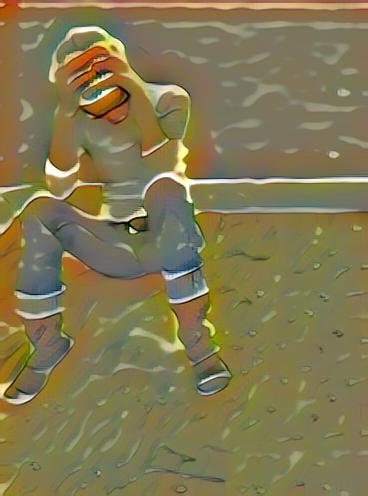
\includegraphics[width=0.17\textwidth]{content1_style1_style3.jpg}
    }
    \subfigure[$\lambda = 10$]{
        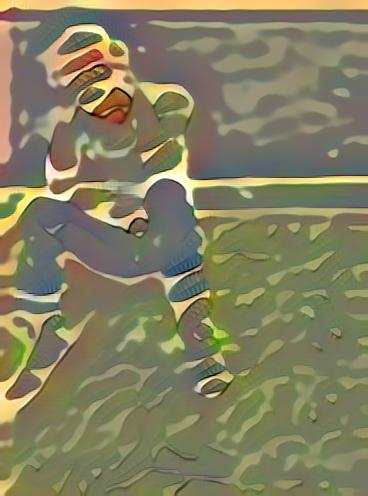
\includegraphics[width=0.17\textwidth]{content1_style1_style10.jpg}
    }\\
    \subfigure[原内容图像]{
        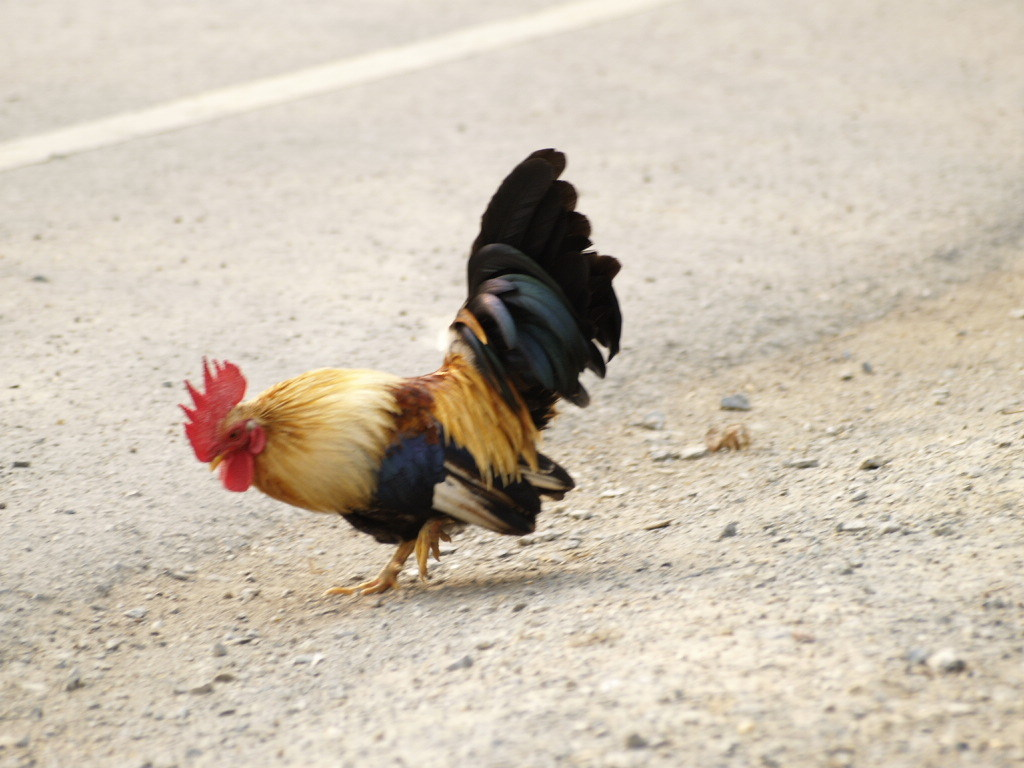
\includegraphics[width=0.17\textwidth]{content2.jpg}
    }
    \subfigure[$\lambda = \frac{1}{3}$]{
        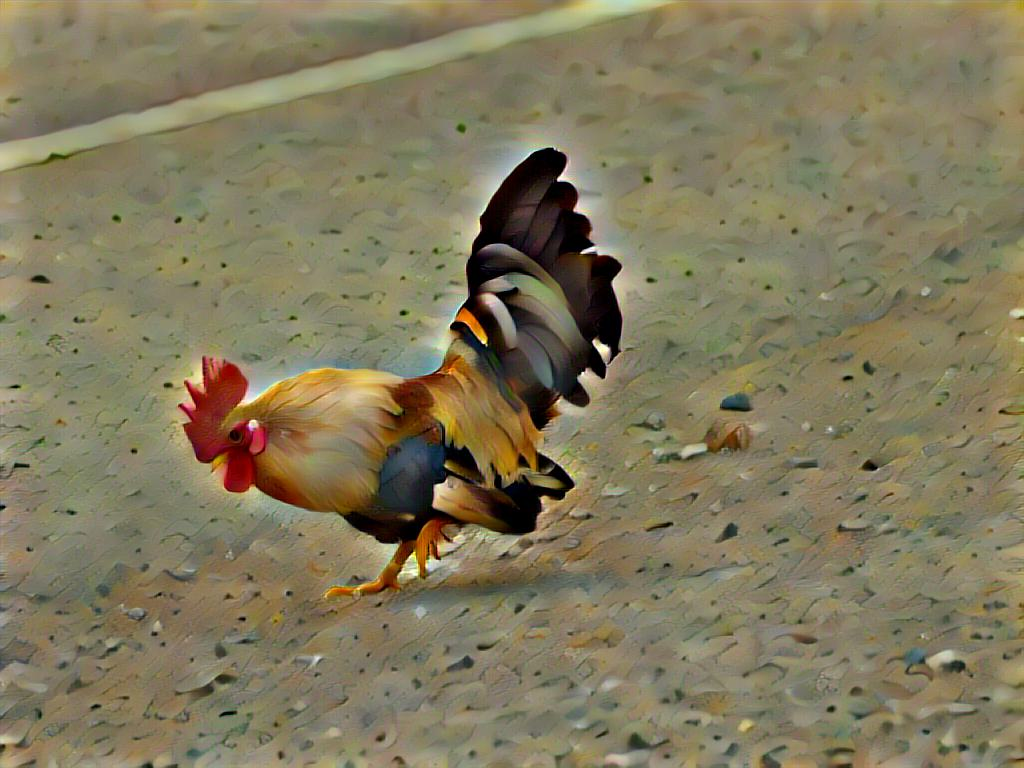
\includegraphics[width=0.17\textwidth]{content2_style1_content3.jpg}
    }
    \subfigure[$\lambda = 1$]{
        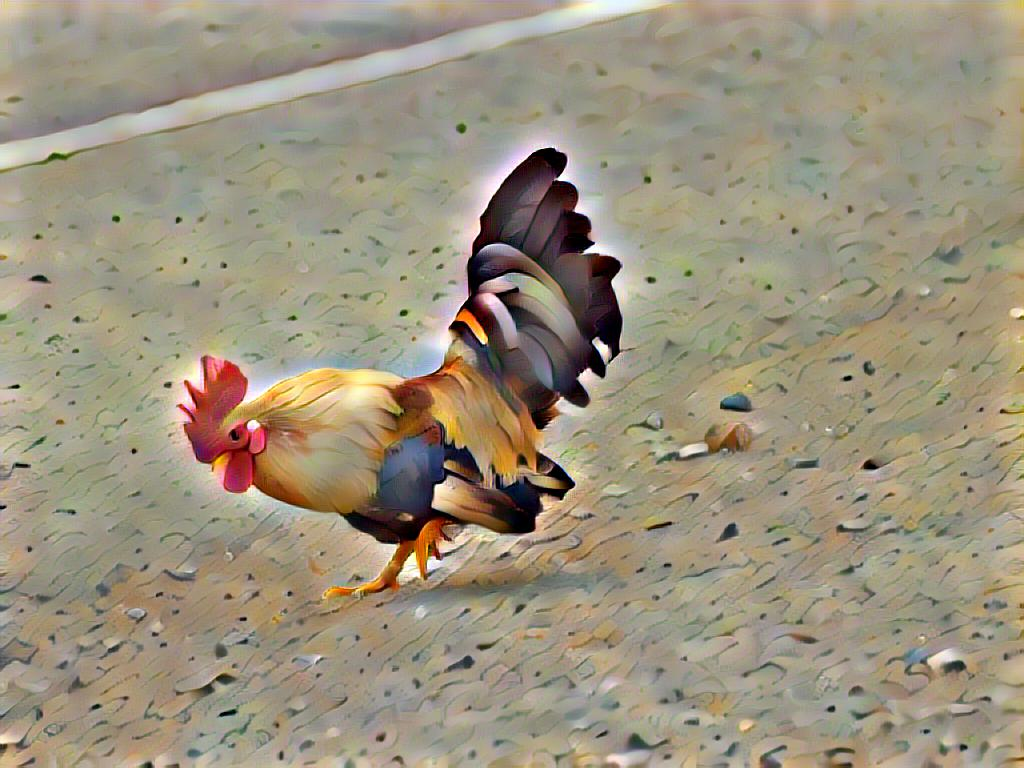
\includegraphics[width=0.17\textwidth]{content2_style1_style1.jpg}
    }
    \subfigure[$\lambda = 3$]{
        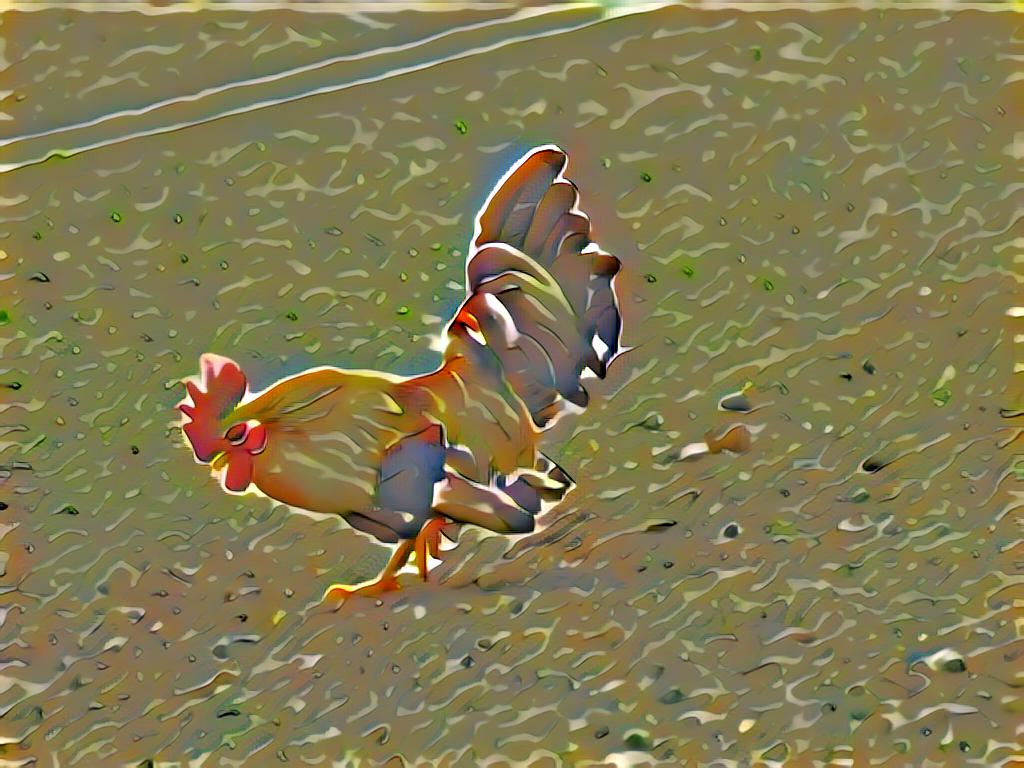
\includegraphics[width=0.17\textwidth]{content2_style1_style3.jpg}
    }
    \subfigure[$\lambda = 10$]{
        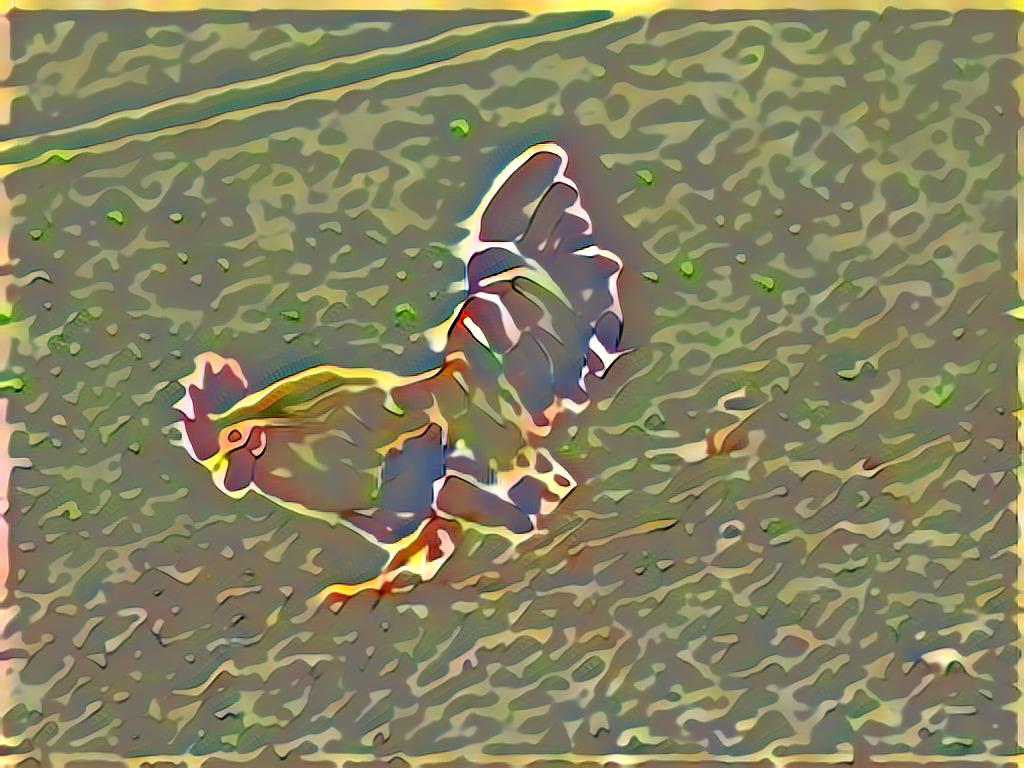
\includegraphics[width=0.17\textwidth]{content2_style1_style10.jpg}
    }\\
    \subfigure[原内容图像]{
        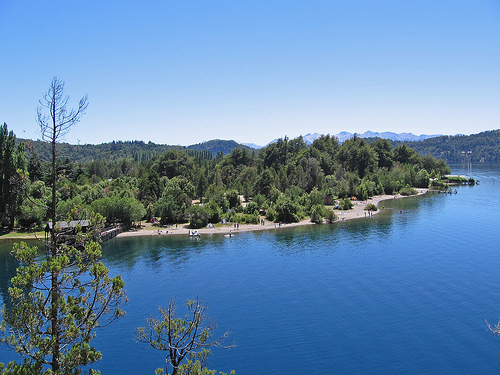
\includegraphics[width=0.17\textwidth]{contents3.jpg}
    }
    \subfigure[$\lambda = \frac{1}{3}$]{
        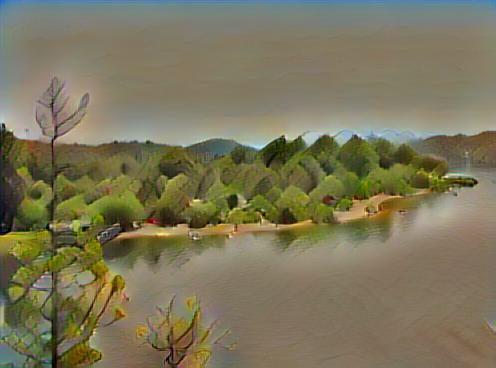
\includegraphics[width=0.17\textwidth]{content3_style1_content3.jpg}
    }
    \subfigure[$\lambda = 1$]{
        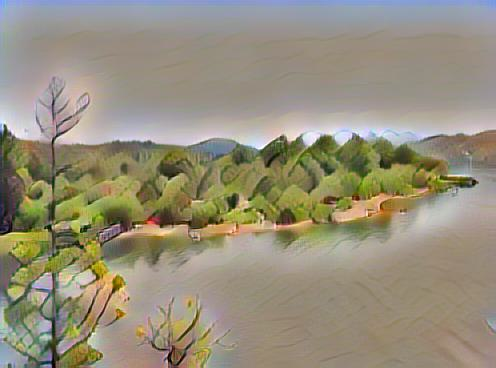
\includegraphics[width=0.17\textwidth]{content3_style1_style1.jpg}
    }
    \subfigure[$\lambda = 3$]{
        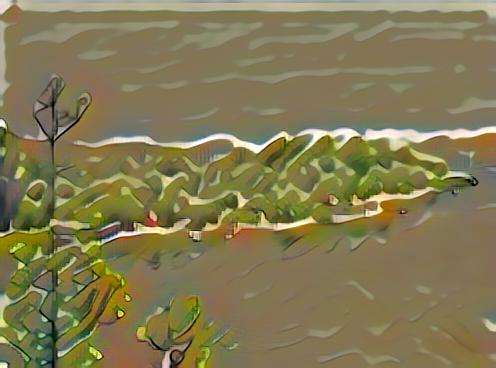
\includegraphics[width=0.17\textwidth]{content3_style1_style3.jpg}
    }
    \subfigure[$\lambda = 10$]{
        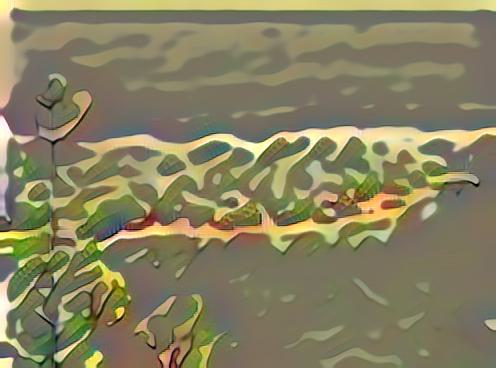
\includegraphics[width=0.17\textwidth]{content3_style1_style10.jpg}
    }\\
    \subfigure[原内容图像]{
        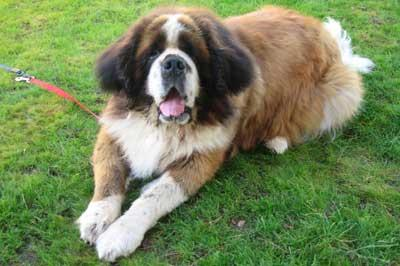
\includegraphics[width=0.17\textwidth]{content4.jpg}
    }
    \subfigure[$\lambda = \frac{1}{3}$]{
        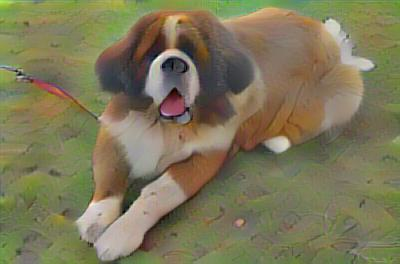
\includegraphics[width=0.17\textwidth]{content4_style1_content3.jpg}
    }
    \subfigure[$\lambda = 1$]{
        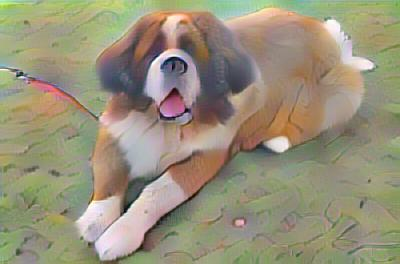
\includegraphics[width=0.17\textwidth]{content4_style1_style1.jpg}
    }
    \subfigure[$\lambda = 3$]{
        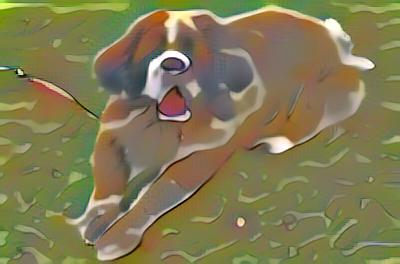
\includegraphics[width=0.17\textwidth]{content4_style1_style3.jpg}
    }
    \subfigure[$\lambda = 10$]{
        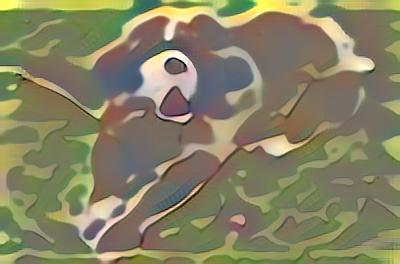
\includegraphics[width=0.17\textwidth]{content4_style1_style10.jpg}
    }
    \caption{不同内容图像和风格图像1下,不同$\lambda$值的风格迁移结果}
    \label{fig:style1}
\end{figure}

\section{实验结果}

为了验证模型的效果,我们通过调整风格损失的权重系数 $\lambda$ ,训练了多个模型,来观察生成图像的风格迁移效果。$\lambda$ 的值越大,生成图像的风格越接近于风格图像;反之,生成图像的内容结构越接近于内容图像。$\lambda$ 的取值为 $[\frac{1}{3}, 1, 3, 10]$,在后续展示图片时,模型的顺序也是按照 $\lambda$ 的值从小到大排列的。为了尽可能不引入浮点计算,对于$\lambda = \frac{1}{3}$,我们采用了$\mathcal{L} = 3 \cdot \mathcal{L}_c + \mathcal{L}_s$
。我们在训练过程中记录了每个模型的内容损失和风格损失,并绘制了每个模型的总损失曲线$\mathcal{L}_\lambda$,如图~\ref{fig:loss}所示。同时,每一个模型的训练时间也被记录在表~\ref{tab:lambda_time_transposed}中。

我们选择了5张内容图像和2张风格图像来测试我们训练好的模型。内容图像将被展示于结果图的第一列,风格图像展示在图~\ref{fig:styles}中。

如图~\ref{fig:style1}和图~\ref{fig:style2}所示,我们展示了不同内容图像和风格图像下,不同 $\lambda$ 值的风格迁移结果。每一行展示的是同一张内容图像在不同 $\lambda$ 值下的风格迁移结果,第一列为原内容图像,第二列为 $\lambda = \frac{1}{3}$ 的结果,第三列为 $\lambda = 1$ 的结果,第四列为 $\lambda = 3$ 的结果,第五列为 $\lambda = 10$ 的结果。



\begin{figure}[t]
    \centering
    \subfigure[原内容图像]{
        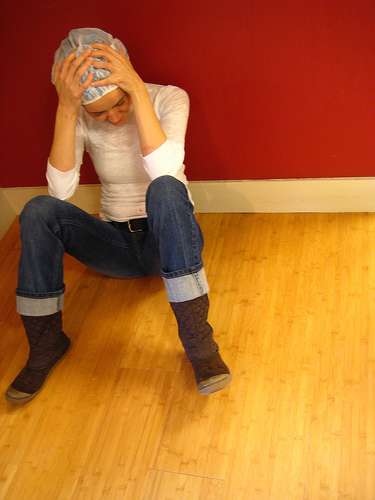
\includegraphics[width=0.17\textwidth]{content1.jpg}
    }
    \subfigure[$\lambda = \frac{1}{3}$]{
        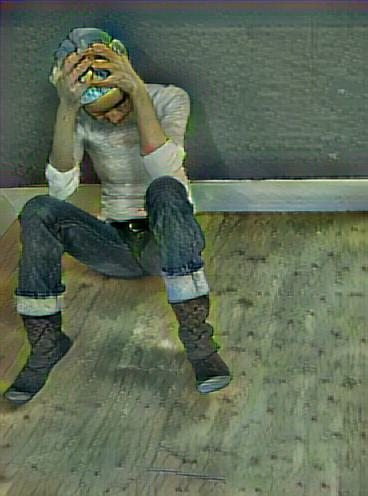
\includegraphics[width=0.17\textwidth]{content1_style2_content3.jpg}
    }
    \subfigure[$\lambda = 1$]{
        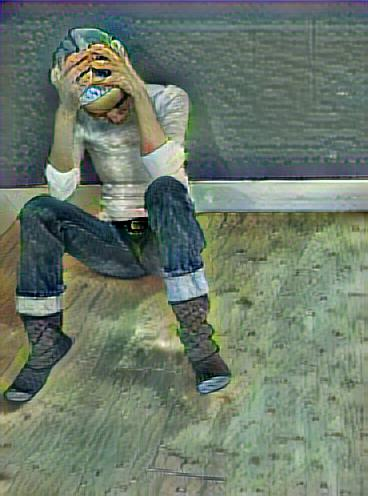
\includegraphics[width=0.17\textwidth]{content1_style2_style1.jpg}
    }
    \subfigure[$\lambda = 3$]{
        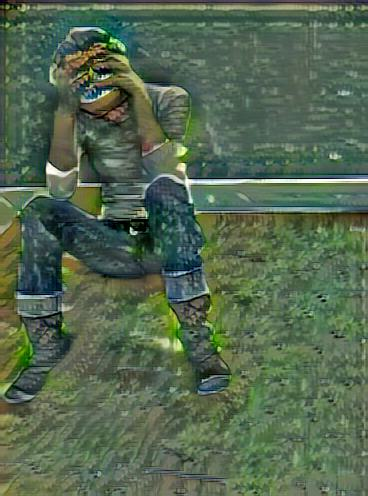
\includegraphics[width=0.17\textwidth]{content1_style2_style3.jpg}
    }
    \subfigure[$\lambda = 10$]{
        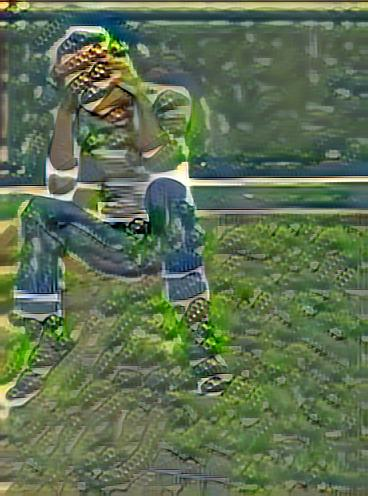
\includegraphics[width=0.17\textwidth]{content1_style2_style10.jpg}
    }\\
    \subfigure[原内容图像]{
        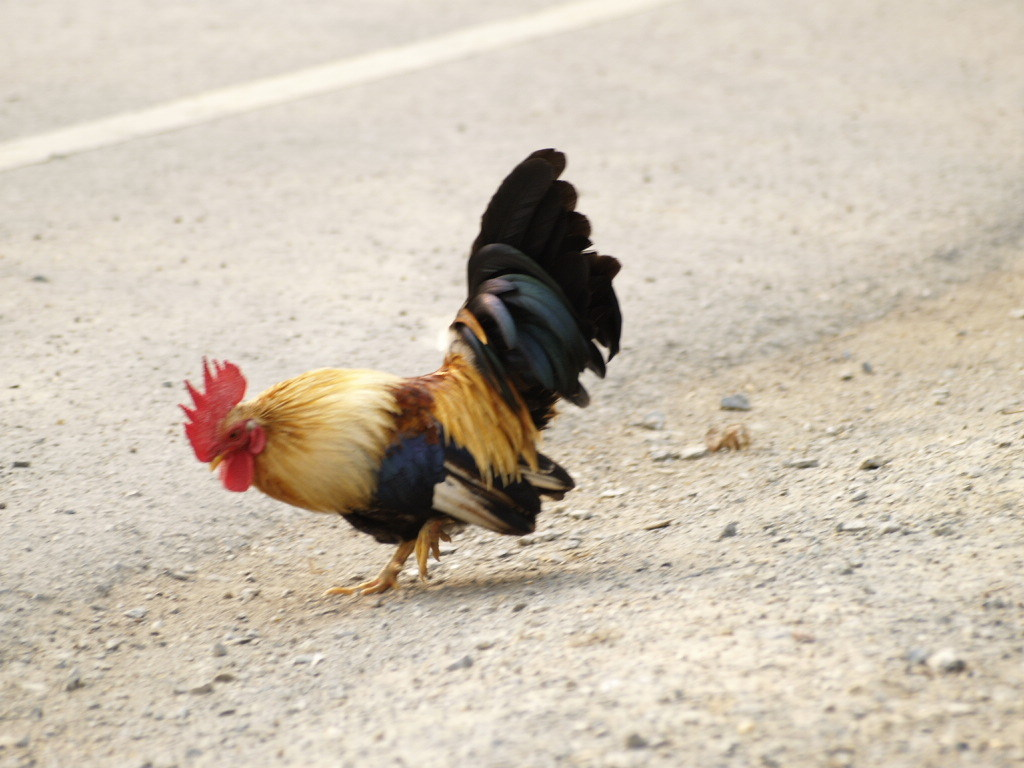
\includegraphics[width=0.17\textwidth]{content2.jpg}
    }
    \subfigure[$\lambda = \frac{1}{3}$]{
        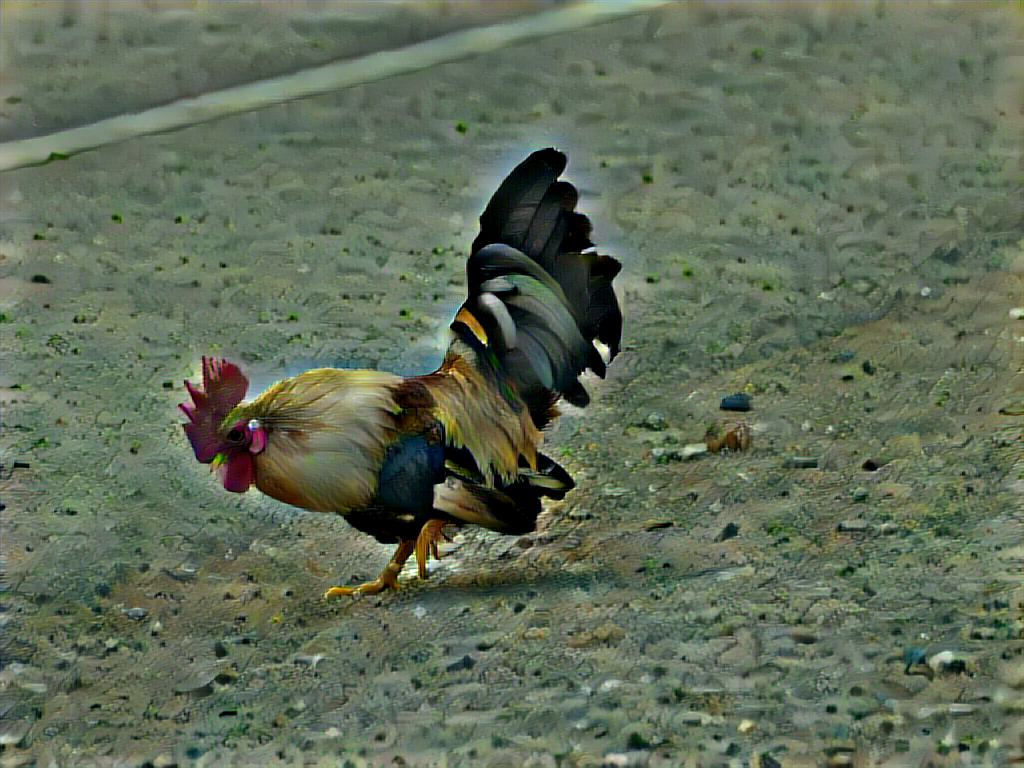
\includegraphics[width=0.17\textwidth]{content2_style2_content3.jpg}
    }
    \subfigure[$\lambda = 1$]{
        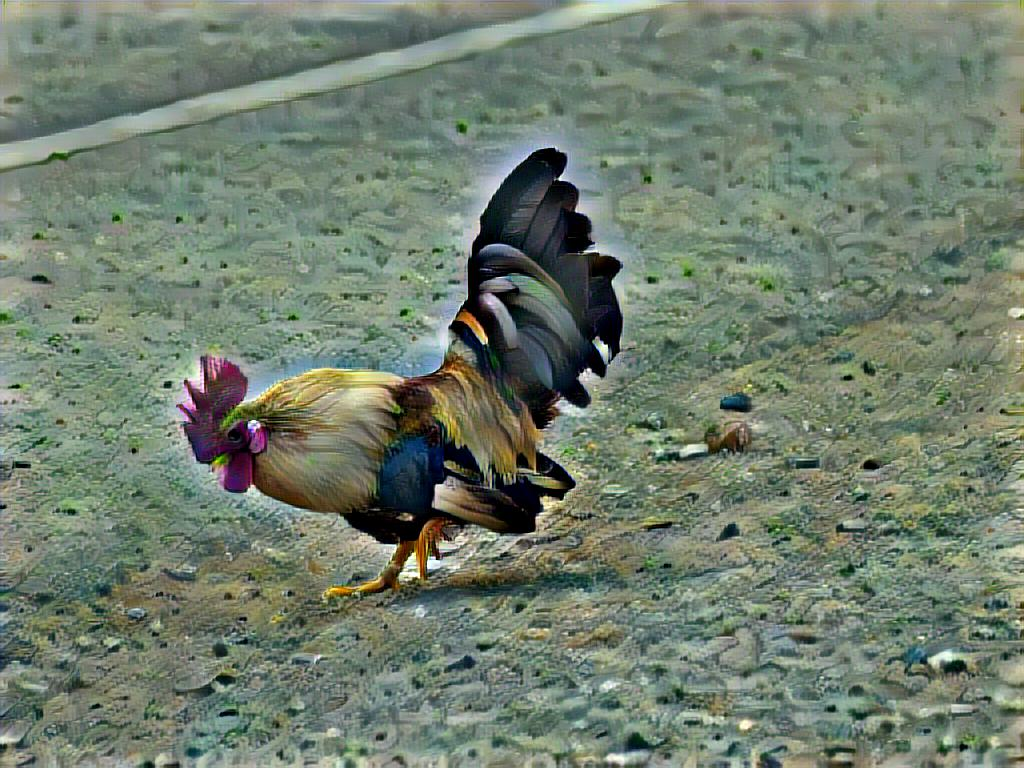
\includegraphics[width=0.17\textwidth]{content2_style2_style1.jpg}
    }
    \subfigure[$\lambda = 3$]{
        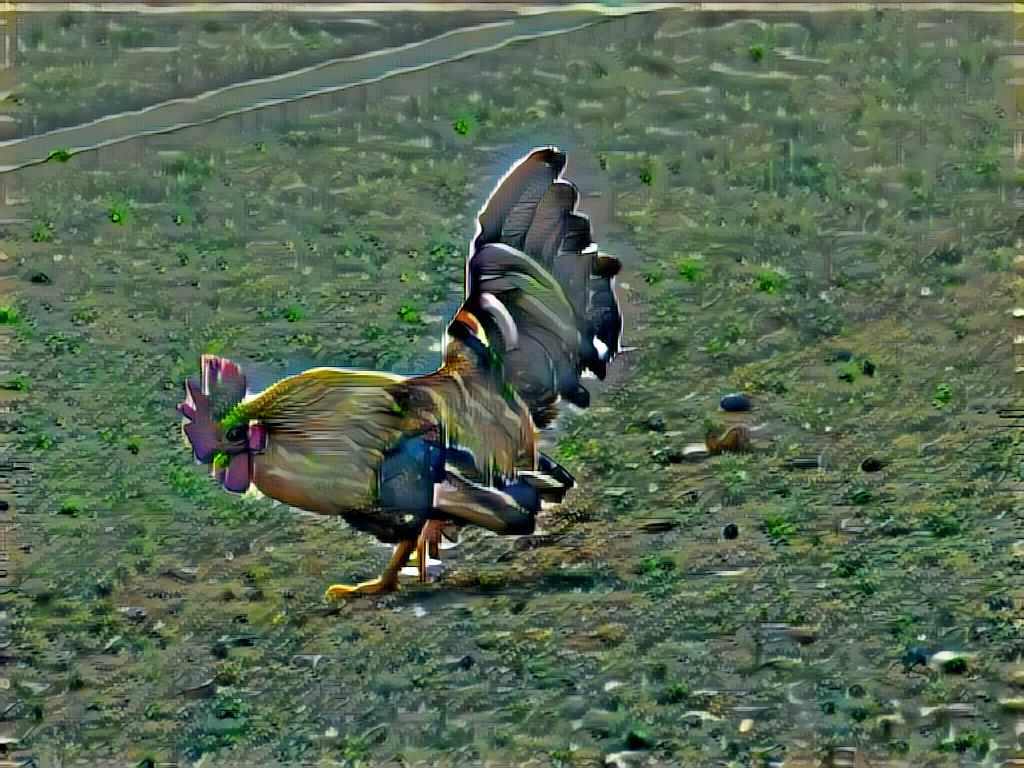
\includegraphics[width=0.17\textwidth]{content2_style2_style3.jpg}
    }
    \subfigure[$\lambda = 10$]{
        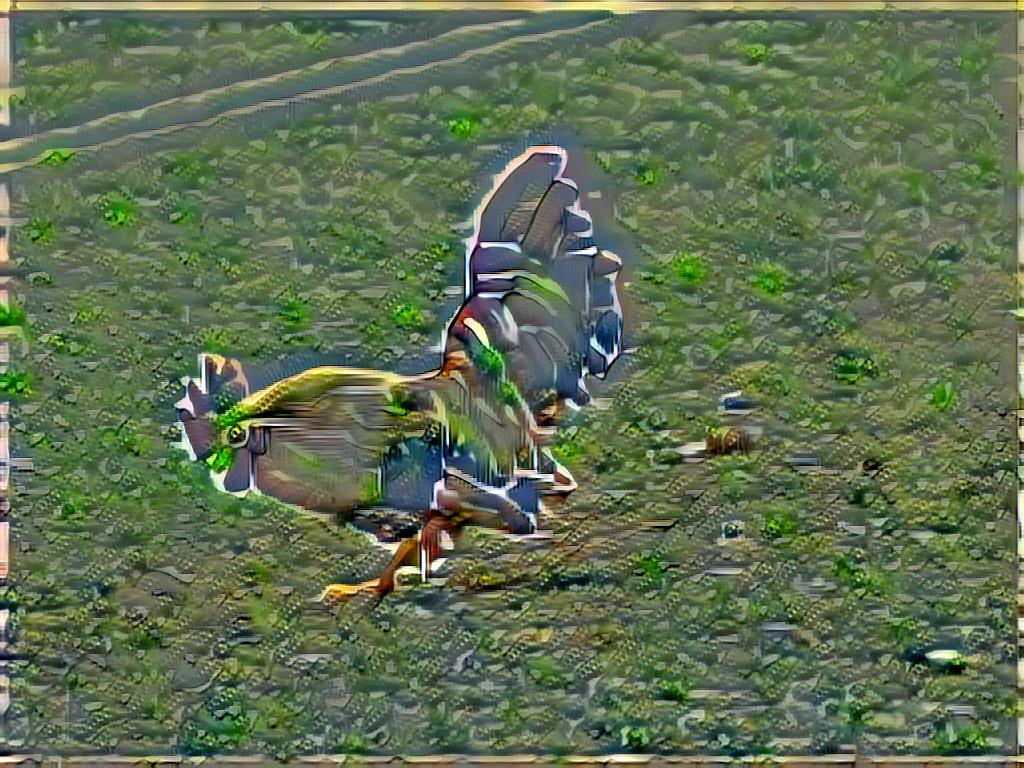
\includegraphics[width=0.17\textwidth]{content2_style2_style10.jpg}
    }\\
    \subfigure[原内容图像]{
        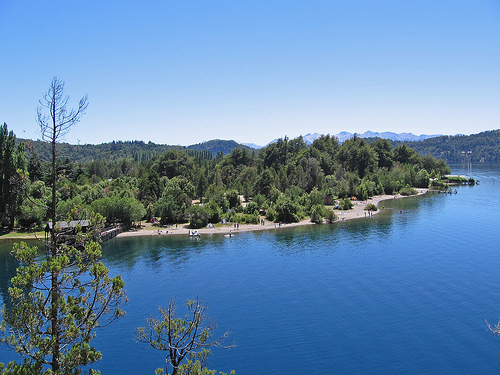
\includegraphics[width=0.17\textwidth]{contents3.jpg}
    }
    \subfigure[$\lambda = \frac{1}{3}$]{
        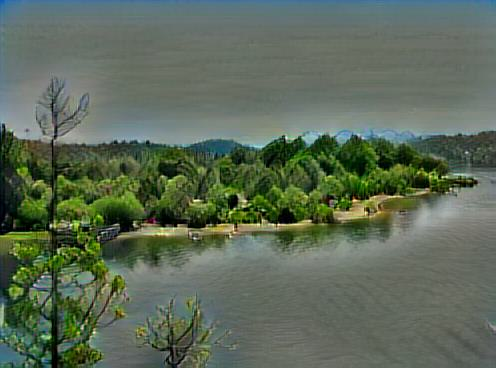
\includegraphics[width=0.17\textwidth]{content3_style2_content3.jpg}
    }
    \subfigure[$\lambda = 1$]{
        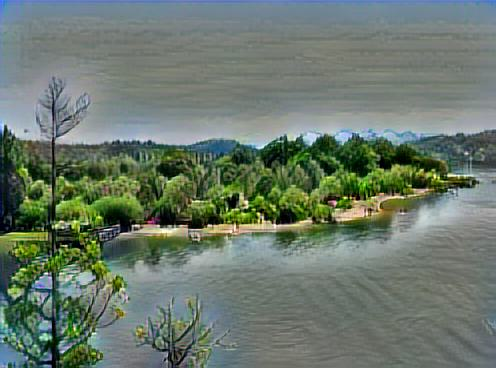
\includegraphics[width=0.17\textwidth]{content3_style2_style1.jpg}
    }
    \subfigure[$\lambda = 3$]{
        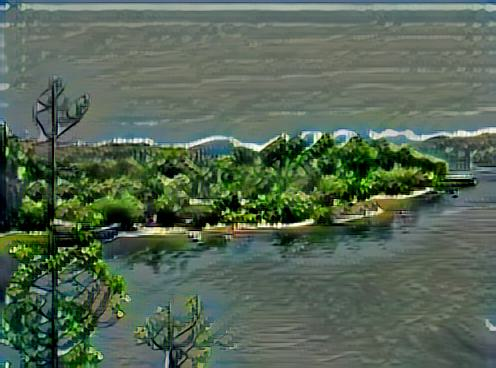
\includegraphics[width=0.17\textwidth]{content3_style2_style3.jpg}
    }
    \subfigure[$\lambda = 10$]{
        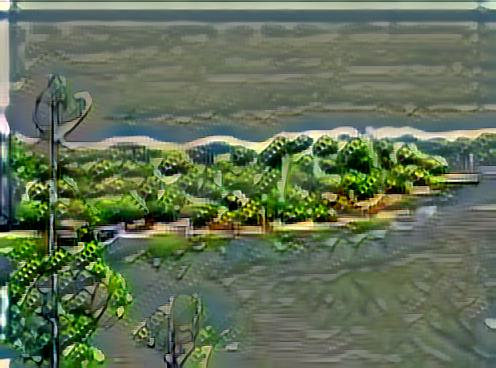
\includegraphics[width=0.17\textwidth]{content3_style2_style10.jpg}
    }\\
    \subfigure[原内容图像]{
        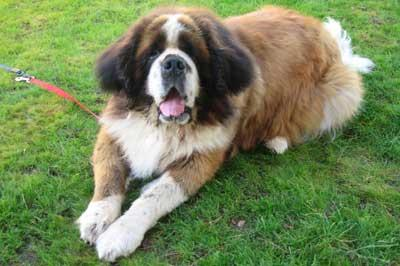
\includegraphics[width=0.17\textwidth]{content4.jpg}
    }
    \subfigure[$\lambda = \frac{1}{3}$]{
        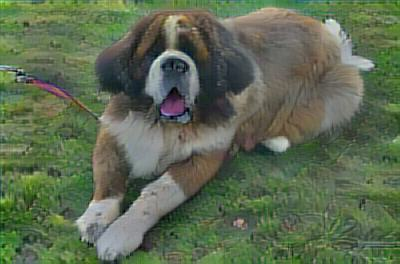
\includegraphics[width=0.17\textwidth]{content4_style2_content3.jpg}
    }
    \subfigure[$\lambda = 1$]{
        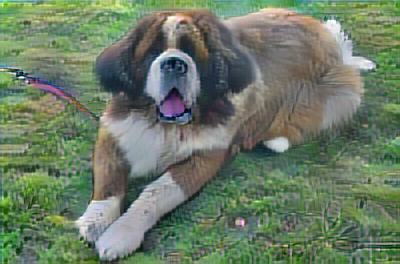
\includegraphics[width=0.17\textwidth]{content4_style2_style1.jpg}
    }
    \subfigure[$\lambda = 3$]{
        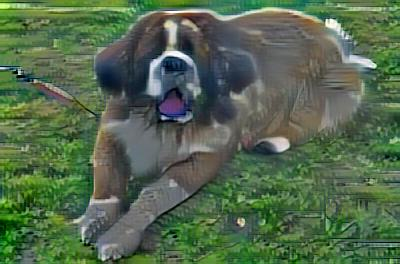
\includegraphics[width=0.17\textwidth]{content4_style2_style3.jpg}
    }
    \subfigure[$\lambda = 10$]{
        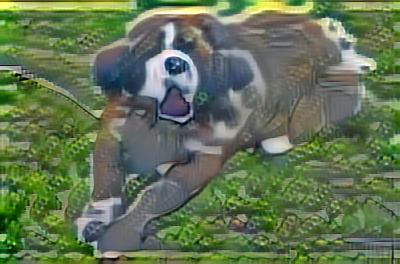
\includegraphics[width=0.17\textwidth]{content4_style2_style10.jpg}
    }
    \caption{不同内容图像和风格图像2下,不同$\lambda$值的风格迁移结果}
    \vspace{-3ex}
    \label{fig:style2}
\end{figure}

可以看到,随着 $\lambda$ 的增大,生成图像的风格逐渐接近于风格图像,而内容结构则逐渐被模糊化。$\lambda = \frac{1}{3}$ 时,生成图像的内容结构较为清晰,但风格特征较弱;而 $\lambda = 10$ 时,生成图像的风格特征明显,但内容结构几乎完全被覆盖。我们发现,$\lambda = 1$ 或 $\lambda = 3$ 时,生成图像的内容和风格特征相对来说较为平衡,能够较好地保留内容结构的同时融合风格特征。

\chapter{实验总结}

本次实验实现了基于自适应实例归一化(AdaIN)的图像风格迁移模型,通过结合内容图像的结构和风格图像的艺术特征,成功生成了高质量的风格迁移图像。模型利用VGG19提取特征,并通过内容损失和风格损失优化图像生成过程。实验结果表明,该模型能够有效地平衡内容和风格之间的融合,生成比较具有动漫风格的图像。这加深了我们对深度学习模型在图像处理任务中的应用理解。

\bibliographystyle{plain}
\bibliography{reference}

\end{document}